\documentclass[]{article}
\usepackage{fullpage}
\usepackage{amsfonts}
\usepackage{amsmath}
\usepackage{amssymb}
\usepackage{graphicx}
\usepackage{tikz}
\usepackage{amssymb}
\let\oldemptyset\emptyset
\let\emptyset\varnothing
\begin{document}


	\title{MAT 1341}
	\author{{\bf Introduction to Linear Algebra}}
	\date{2013}
	\maketitle

	\begin{center}
		{\bf Professor:} Wanshun Wong\\
	\end{center}
	\pagebreak
	\Large{Chapter 2: Complex Numbers}\\
	\large{\bf 2.1 defining the complex numbers}\\\\
	\noindent
	\normalsize
		The equation $x^2+1=0$ has no solutions in $\mathbb{R}$.\\
		Let $i=\sqrt{-1} \ \ \ \ \ (\star)$\\
		Then $i^2=-1$, hence $i^2+1=0$.\\
		Hence $i$ is a solution to $(\star)$.\\\\
		Example: consider $x^2+2x+2=0$\\
		By the quadratic formula, the solutions are:
		$$x=\frac{-2\pm\sqrt{4-8}}{2}=\frac{-2\pm\sqrt{-4}}{2}=\frac{-2\pm 2\sqrt{-1}}{2}={\bf-1\pm i}$$
		Check:
		$$(-1+i)^2=(-1+i)(-1+i)=1-2i-1={\bf -2i}$$
		Hence:
		$$(-1+i)^2+2(-1+i)+2=-2i-2+2i+2={\bf 0}$$
		\\\\
		\begin{description}
			\item[Definition] \hfill \\
				The set of complex numbers is $\mathbb{C}=\{a+bi~|~a,b\in\mathbb{R}\}$\\
				When we write $z=a+bi$, where $a, b\in\mathbb{R}$:
				\begin{itemize}
					\item $a$ is called the real part, and is denoted by $Re(z)$, and
					\item $bi$ is called the imaginary part, and is denoted by $Im(z)$.
				\end{itemize}
				When $a=0$, $z$ is called  \emph{purely imaginary}.\\
				When $b=0$, $z\in\mathbb{R}$.
		\end{description}
		\begin{center}
			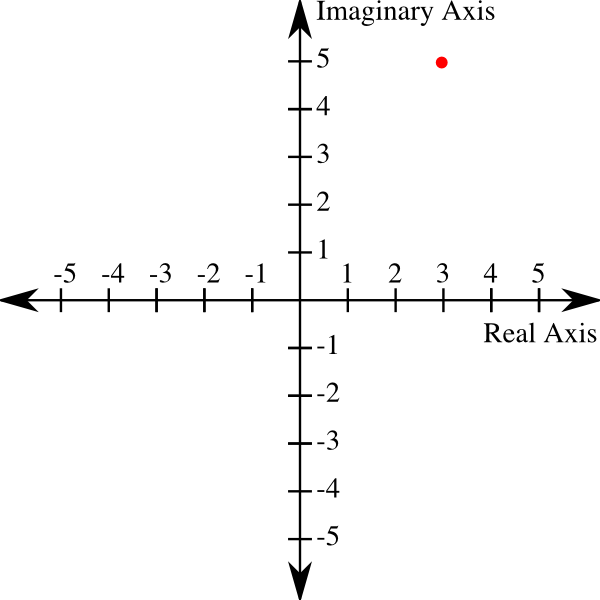
\includegraphics{./graphics/fig002.png}\\
			\emph{The complex plane. The red dot is 3+5i.}
		\end{center}\pagebreak
		
		\noindent{\bf Properties of complex numbers}\\
		If $z$, $w$, $y\in\mathbb{C}$:
		\begin{itemize}
			\item $z+w=w+z$
			\item $zw=wz$
			\item $1\times z=z$
			\item $0\times z=0$
			\item $y(z+w)=yz+yw$
			\item $y(zw)=(yz)w$
		\end{itemize}
		Given any quadratic equation $ax^2+bx+c$ where $\{a\ne 0\ |\ a, b, c\in\mathbb{R}\}$,\\
		the solutions are found using $x=\frac{-b\pm\sqrt{b^2-4ac}}{2a}$.
		If $b^2-4ac\ge 0$, the solutions $\in\mathbb{R}$.\\
		If $b^2-4ac<0$, the solutions are complex.\\\\
		\large{\bf 2.2 Algebra of the complex numbers}\\
		\normalsize
		For $a$, $b$, $c\in\mathbb{R}$:
		\begin{itemize}
			\item $a+bi=c=di\Leftrightarrow a=c$ and $b=d$
			\item $(a+bi)+(c+di)=(a+c)+(b+d)i$
			\item $(a+bi)(c+di)=ac-bd$
		\end{itemize}
		\begin{description}
			\item[Definition] \hfill\\
				The {\bf complex conjugate} of $z=a+bi$ is $\overline{z}=a-bi$.
			\item[Example]\hfill\\
				$\overline{1+2i}=1-2i$\\
				$z\overline{z}=\overline{z}z$\\
				$=(a+bi)(a-bi)$\\
				$=a^2+b^2$
		\end{description}
		$z$ is a nonnegative, real number.\\
		The absolute value of $z$ is $|z|=\sqrt{a^2+b^2}=\sqrt{z\overline{z}}$
		\begin{itemize}
			\item $z=0\Leftrightarrow a-b=0\Leftrightarrow |z|=0$
			\item $\frac{1}{z}=\frac{1}{z}\times\frac{\overline{z}}{z}$\\
				$=\frac{\overline{z}}{|z^2|}$\\
				$=\frac{1}{a+bi}=\frac{a-bi}{a^2+b^2}$\\
				$=\frac{a}{a2+b2}-\frac{b}{a2+b2}i$\\
		\end{itemize}
		\begin{description}
			\item[Example]\hfill\\\\
			$\frac{1}{1+i}=\frac{1}{1-i}\times\frac{1-i}{1-i}$\\\\
			$=\frac{1-i}{1^2+1^2}$\\\\
			$=\frac{1-i}{2}=\frac{1}{2}-\frac{1}{2}i$
			\item[Example]\hfill\\\\
			$\frac{2+i}{1-3i}=\frac{2+i}{1-3i}\times\frac{1+3i}{1+3i}$\\\\
			$=\frac{(2-3)+(6+1)i}{1^2+3^2}$\\\\
			$=\frac{-1}{10}+\frac{7}{10}i$\\\\
		\end{description}
		
		\noindent\large{\bf 2.3 Geometry of the complex numbers}\\
		\normalsize Numbers on the complex plane may be treated as vectors when performing addition, with the real and complex parts corresponding to coordinates.
		\begin{itemize}
			\item Multiplication by a real corresponds to scaling
			\item $|z|=$ length of a vector, e.g. $|2+i|=\sqrt{2^2+1^2}=\sqrt{5}$
		\end{itemize}
		
		\noindent\large{\bf 2.4 Polar form of complex numbers}\\
		\normalsize $z=a+bi$\\
		$r=|z|=\sqrt{a^2+b^2}$\\
		$\cos\theta=\frac{a}{r}$\\
		$\sin\theta=\frac{b}{r}$\\
		Polar form of $z$:\\
		$z=a+bi=(r\cos\theta)+(r\sin\theta)i$\\
		$=r(\cos\theta+i\sin\theta)$\\\\
		
		Note that $\theta=\arg(z)\rightarrow$ argument of $z$ is not uniquely determined since $\theta+2n\pi$ also works for any $n\in\mathbb{Z}$.\\
		We usually pick $-\pi<\theta\le\pi$ and write $\theta=\arg(z)$, principal argument of $z$.\\
		
		\begin{description}
			\item[Recall]\hfill\\
				$e^z=i+z+\frac{z}{2}+\frac{z}{4}+...=\sum\limits^\infty_{n=0}\frac{z^n}{n!}$\\
				$e^{i\theta}=\cos\theta+i\sin\theta$\\
				So we can write\\
				$z=re^{i\theta}$
			\item[Properties]\hfill\\
				$re^{i\theta}=se^{i\phi}\Leftrightarrow r=s$ and $\theta=\phi+2n$ for some integer $n$.\\\\
				$\overline{re^{i\theta}}=re^{-i\theta}$\\
				$|e^{i\theta}|=1$ for any $\theta$\\
		\end{description}
		\noindent\large{\bf 2.5 Multiplying complex numbers in polar form}
		\normalsize
		\begin{description}
			\item[If $z=re^{i\theta}$, $w=se^{i\phi}$]\hfill\\
				$zw=r(\cos\theta+i\sin\theta)\times s(\cos\phi+i\sin\phi)$\\
				$=rs[(\cos\theta\cos\phi-\sin\theta\sin\phi)+(\sin\theta\cos\phi+\cos\theta\sin\phi)i]$\\
				$=rs[\cos(\theta+\phi)+i\sin(\theta+\phi)]$\\
				$=rse^{i(\theta+\phi)}$
			
			\item[Example]\hfill\\
				$1+i=\sqrt{2}e^{-i\frac{\pi}{4}}$\\
				hence\\
				$\frac{1}{1+i}=\frac{1}{\sqrt{2}}e^{-i\frac{\pi}{4}}$
		\end{description}

		\noindent\large{\bf 2.6 Fundamental theorem of algebra}\\
		\normalsize
		\noindent Every polynomial with coefficients in the complex numbers can be factored completely into linear factors of the for $zx+w$, with $z$, $w\in\mathbb{C}$.\\
		\begin{description}
			\item[Example]\hfill\\
				$x^2+1=(x+i)(x-i)$
		\end{description}
		Every degree $n$ polynomial with coefficients in the complex plane has $n$ solutions (counting multiplicities).\\\\
		\pagebreak\\
		\Large{Chapter 3: Vector geometry}\\
		\noindent\normalsize
		{\bf 3.1\\} 
		Algebra $\longleftrightarrow$ Geometry\\
		$\mathbb{R}$~~~~~~~~~~~~~~~~line\\
		$\mathbb{R}^2$~~~~~~~~~~~~~~~plane\\
		$\mathbb{R}^3$~~~~~~~~~~~~~~~3-plane\\
		$\mathbb{R}^n$~~~~~~~~~~~~~~~n-space\\\\
		Notations:\\
		$\vec{x}=(1,2,3)$\\
		$\vec{x}=\underline{i},\underline{2j},\underline{3k}$\\
		$\vec{x}=
		\begin{bmatrix}
			{1}\\
			{2}\\
			{3}
		\end{bmatrix}=[1,2,3]$\\
		$\mathbb{R}^n=\{(x_1,...x_n~|~x_1,...,x_n\in\mathbb{R} \}$\\\\
		{\bf 3.2 Properties}
		\begin{itemize}
			\item $(x_1,~...,~x_n)=(y_1,~...,~y_n)\Leftrightarrow x_1=y_1,~x_n=y_n$
			\item $(x_1,~...,~x_n)+(y_1,~...,~y_n)=(x_1+y_1,~...,~x_n+y_n)$
			\item $\vec{0}=(0,~...,~0)\in\mathbb{R}^n$
			\item if $\vec{x}=(x_1,~...,~x_n)$, then $-\vec{x}=(-x_1,~...,~-x_n)$ and $\vec{x}+(-\vec{x})=\vec{0}$
			\item if $r\in\mathbb{R},~\vec{x}=(x_1,~...,~x_n)\in\mathbb{R}^n$, then $r\cdot\vec{x}=(rx, ~rx_2,~...,~rx_n)$			
			\item 2 vectors are equal $\iff$ they have the same magnitude and same direction
			\item Head-to-tail rule
			\item $\vec{0}$ is te only vector with 0 magnitude.
			\item negative=reverse direction
			\item 2 vectors are parallel$\iff$they are multiples of eachother
		\end{itemize}
		\pagebreak
		{\bf 3.3 Definition:}\\
		If $r_1,~...,~r_n\in\mathbb{R}$,\\
		$\vec{x_1},~...,~\vec{x_n}\in\mathbb{R}^n$\\
		then $\vec{y}=r_1\vec{x_1}+...+r_n\vec{x_n}$ is a \emph{linear combination} of $\vec{x_1},~...,\vec{x_n}$\\
		We are looking for two scalars, $r_1,~r_2\in\mathbb{R}$, such that\\
		$$\begin{bmatrix}
			{3}\\
			{3}\\
			{4}\\
		\end{bmatrix}=r_1
		\begin{bmatrix}
			{1}\\
			{2}\\
			{2}\\
		\end{bmatrix}+r_2
		\begin{bmatrix}
			{1}\\
			{1/2}\\
			{0}\\
		\end{bmatrix}
		$$\\
		$$
		 \begin{cases}
			3=r_1+r_2\\
			3=2r_1+\frac{1}{2}r_2\\
			4=3r_1
		\end{cases}
		$$
		But $3\ne 2(\frac{4}{3})+\frac{1}{5}(\frac{5}{3})$\\\\
		{\bf 3.4 More properties}\\
		$r,~s\in\mathbb{R},~\vec{u},~\vec{v},~\vec{w}\in\mathbb{R}^n$
		\begin{itemize}
			\item $(\vec{u}+\vec{v})+\vec{w}=\vec{u}+(\vec{v}+\vec{w})$
			\item $\vec{u}+\vec{0}=\vec{u}$
			\item $\vec{u}+(-\vec{u})=\vec{0}$
			\item $r(\vec{u}+\vec{v})=r\vec{u}+r\vec{v}$
			\item $(r+s)\vec{u}=r\vec{u}+s\vec{u}$
			\item $(rs)\vec{u}=r(s\vec{u})$
			\item $1\cdot\vec{u}=\vec{u}$
		\end{itemize}
		{\bf 3.5 Definition}\\
		The dot product of $\vec{x}=(x_1,~...,~x_n)$ and $\vec{y}=(y_1,~...,~y_n)$ is\\
		$\vec{x}\cdot\vec{y}=x_1y_1+x_2y_2+...+x_ny_n$\\
		And the norm of $\vec{x}$ is $||\vec{x}||=\sqrt{\vec{x}\cdot\vec{x}}\\=\sqrt{x_1^2+...+x_n^2}$
		Note that $||\vec{x}||=0\iff\vec{x}=\vec{0}$\\\\
		{\bf 3.6 Definition}\\
		if $\vec{x}\cdot\vec{y}\in\mathbb{R}^n$\\
		then $\vec{x}$ and $\vec{y}$ are said to be \emph{orthogonal} (perpendicular), and $\vec{x}\cdot\vec{y}=0$\\\\
		{\bf 3.7: The Cauchy-Schwarz Inequality}\\
		let $\vec{u},~\vec{v}\in\mathbb{R}^n$\\
		then $|\vec{u}\cdot\vec{v}|\le||\vec{u}||~||\vec{v}||$\\
		$||\vec{u}+\vec{v}||^2=(\vec{u}+\vec{v})\cdot(\vec{u}+\vec{v})$\\
		$=||\vec{u}||^2+2\vec{u}\vec{v}+||\vec{v}||^2$\\
		$\le||\vec{u}||^2+2|\vec{u}\vec{v}|+||\vec{v}||^2$\\
		$\le||\vec{u}||^2+2||\vec{u}||~||\vec{v}||+||\vec{v}||^2$\\
		$=(||\vec{u}||+||\vec{v}||)^2$\\
		This implies $||\vec{u}+\vec{v}||\le ||\vec{u}||+||\vec{v}||$, triangle inequality.\\\\
		\pagebreak\\
		{\bf Definition}\\
		let $\vec{u},~\vec{v}\in\mathbb{R}^n$,~~~$\vec{u}$, $\vec{v}\ne\vec{0}$\\
		the angle between $\vec{u}$ and $\vec{v}$ is defined by:\\
		$$\cos\theta=\frac{\vec{u}\cdot\vec{v}}{||\vec{u}||~||\vec{v}||}$$
		With $0\le\theta\le\pi$\\
		$$\cos\theta=(\frac{\vec{u}}{||\vec{u}||})\cdot(\frac{\vec{v}}{||\vec{v}||})$$\\
		{\bf Example}\\
		Compute the angle between\\
		$\vec{v}=(0,2,1,\sqrt{3})$ and $\vec{v}=(\sqrt{3},1,2,0)$\\
		$\cos\theta=\frac{0+2+2+0}{\sqrt{4+1+3}+\sqrt{3+1+4}}=\frac{4}{8}=\frac{1}{2}$\\
		$\theta=\frac{\pi}{3}$\\
		{\bf Remark:} $\vec{u}$ and $\vec{v}$ are orthogonal:\\
		$\iff\vec{u}\cdot\vec{v}=0$\\
		$\iff\cos\theta=\frac{\vec{u}\cdot\vec{v}}{||\vec{u}||~||\vec{v}||}=0$\\
		$\iff\theta=\frac{\pi}{2}$\\\\
		$\vec{u}$ and $\vec{v}$ are parallel:\\
		$\iff\theta=0$ or $\pi$\\
		$\iff\cos\theta=1$ or $-1$\\
		$\iff\vec{u}\cdot\vec{v}=||\vec{u}||~||\vec{v}||$ or $-||\vec{u}||~||\vec{v}||$\\
		i.e. $|\vec{u}\cdot\vec{v}|=||\vec{u}||~||\vec{v}||$\\
		This means that $|\vec{u}\cdot\vec{v}|$ attains its maximum value given by Cauchy-Schwarz Inequality.\\\\
		{\bf Definition}\\
		let $\vec{u}, \vec{v}\in\mathbb{R}^n$, ~~$\vec{u},\vec{v}\ne\vec{0}$\\
		The the projection of $\vec{u}$ onto $\vec{v}$ is\\
		$\text{proj}_{\vec{v}}(\vec{u})=\frac{\vec{u}\cdot\vec{v}}{||\vec{v}||^2}\vec{v}$\\
		$=(\vec{u}\frac{\vec{v}}{||\vec{v}||})\frac{\vec{v}}{||\vec{v}||}$\\\\
		{\bf Properties}
		\begin{itemize}
			\item proj$_{\vec{v}}(\vec{u})$ is parallel to $\vec{v}$
			\item $\vec{u}-$proj$_{\vec{v}}(\vec{u})$ is perpendicular to $\vec{v}$
			\item $\vec{u}=(\vec{u}-\text{proj}_{\vec{v}}(\vec{u}))+$proj$_{\vec{v}}(\vec{u})$
		\end{itemize}
		{\bf Example}\\
		$\vec{v}=(1,0,0)$, $\vec{v}=(2,4,6)$\\
		Then proj$_{\vec{u}}(\vec{v})=\frac{\vec{v}\cdot\vec{u}}{||\vec{u}||^2}\vec{v}$\\
		$=\frac{2}{1^2}(1,0,0)$\\
		$=(2,0,0)$\\\\
		$\vec{w}=(5,0,0)$\\
		proj$_{\vec{w}}(\vec{v})=(2,0,0)$
		\pagebreak\\
		\Large{Chapter 4: Lines and planes}\\
		\normalsize
		{\bf 4.1}\\\\
		\begin{center}
			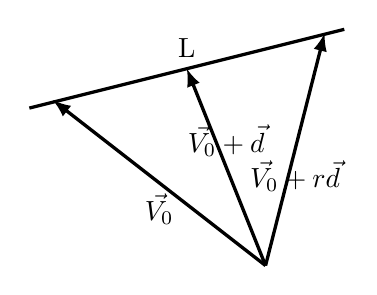
\begin{tikzpicture}
				\draw[very thick](0,0) -- node [above]{L}(4,1);
				\draw[-latex,very thick](3,-2)--node[below]{$\vec{V_0}$}(0.3,0.1);
				\draw[-latex,very thick](3,-2)--node[above]{$\vec{V_0}+\vec{d}$}(2,0.5);
				\draw[-latex,very thick](3,-2)--node[below]{$\vec{V_0}+r\vec{d}$}(3.75,0.95);
			\end{tikzpicture}\\
		\end{center}
		Equation of a line: $y=mx+c$\\\\
		$L=\{\vec{V_0}+r\vec{d}~|~r\in\mathbb{R}\}$\\
		i.e. Any point on L can be written as $\vec{V_0}+r\vec{d}$.\\
		Ex: The line $y=2x+1$ in $\mathbb{R}^2$ can be written as follows:\\
		Let $x=r~\longleftarrow$ parameter\\
		$~~~~~~y=2r+1$
		Then:
		$\begin{bmatrix}
			{x}\\
			{y}
		\end{bmatrix}=
		\begin{bmatrix}
			{r}\\
			{2r+1}
		\end{bmatrix}=
		\begin{bmatrix}
			{0}\\
			{1}
		\end{bmatrix}_{\vec{V_0}}+
		r\begin{bmatrix}
			{1}\\
			{2}
		\end{bmatrix}_{\vec{d}}$\\
		Vector form or parametric form.\\\\
		Ex: Use different letters to represent parameters.\\
		Find the point of intersection of
		$$
			L_1=\{ \begin{bmatrix}{0}\\{1}\end{bmatrix}+r\begin{bmatrix}{1}\\{2}\end{bmatrix}~|~\in\mathbb{R} \}
		$$
		and
		$$
			 L_2=\{ \begin{bmatrix}{1}\\{1}\end{bmatrix}+t\begin{bmatrix}{0}\\{1}\end{bmatrix}~|~\in\mathbb{R} \}
		$$
		Use $t$ for the parameter of $L_2$, and we solve:\\
		$$
		\begin{bmatrix}
			{0}\\
			{1}
		\end{bmatrix}+r
		\begin{bmatrix}
			{1}\\
			{2}
		\end{bmatrix}=
		\begin{bmatrix}
			{1}\\
			{1}
		\end{bmatrix}+r
		\begin{bmatrix}
			{0}\\
			{1}
		\end{bmatrix}
		\begin{cases}
			0+r=1+0\Rightarrow r=1\\
			1+2r=1+r\Rightarrow t=2
		\end{cases}$$
		So the point of intersection is
		$$
		\begin{bmatrix}
			{1}\\
			{3}
		\end{bmatrix}$$\\
		{\bf 4.2}\\
		In $\mathbb{R}$: there is only one line.\\
		In $\mathbb{R}^2$: 2 distinct lines, either parallel or intersecting.\\
		In $\mathbb{R}^3$: 2 distinct lines, either parallel, intersecting, or skew (neither parallel nor intersecting). In the first two cases, there is a unique plane containing both lines.\\
		If they are skew, there is no plane containing both, but there are two \emph{parallel} planes, each containing one line.
		\pagebreak\\
		{\bf 4.3}\\
		\begin{center}
			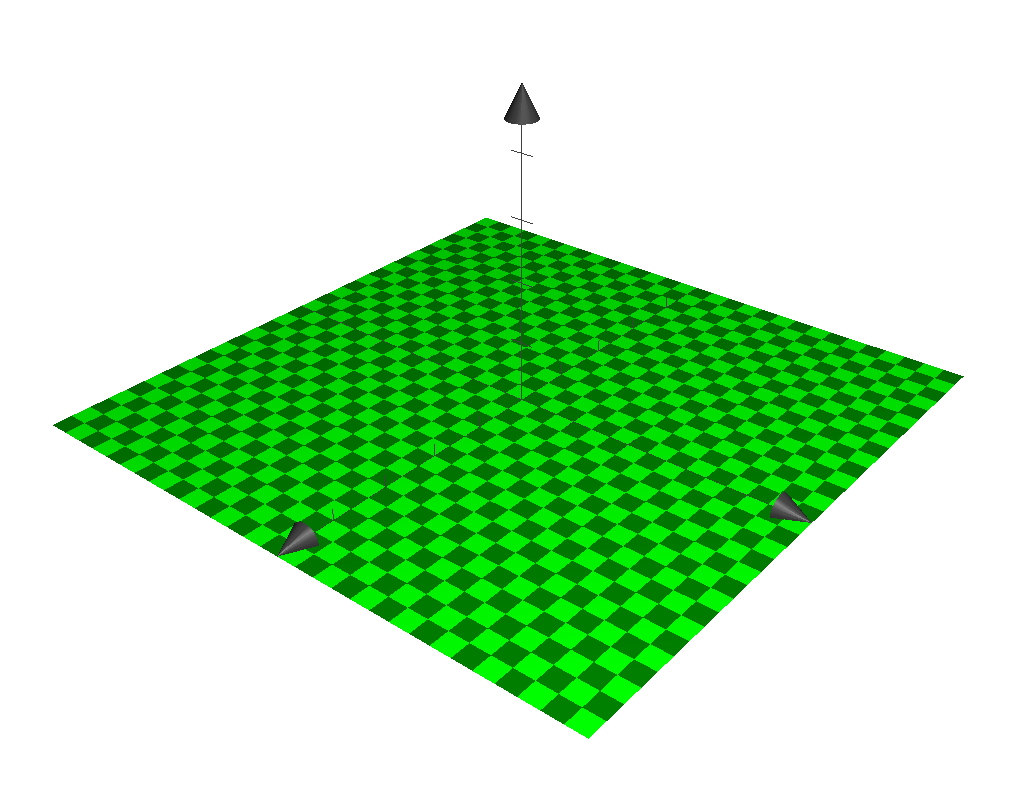
\includegraphics[scale=0.7]{./graphics/plane-1.png}
		\end{center}
		$$
		W=\{ \vec{v}\in\mathbb{R}^3~|~(\vec{v}-\vec{v_0})\cdot\vec{n}=0 \}
		$$
		For example, the plane with $\vec{n}=(1,2,3)$ and containing the point (0,1,1) is:
		$$\{ (x,y,z)\in\mathbb{R}^3~|~[(x,y,z)-(0,1,1)]\cdot(1,2,3)=0 \}$$
		$$(x,y-1,z-1)\cdot(1,2,3)=0$$
		$$x+2y-2+3z-3=0$$
		$$x+2y+3z=5$$\\
		Ex: find the distance from the point (3,3,3) to the plane $x+2y+3z=5$\\
		\begin{align*}
			D&=||\text{proj}_{(1,2,3)}((3,3,3)-(0,1,1))||\\
			&=||\text{proj}_{(1,2,3)}(3,2,2)||\\
			&=|| \frac{3+4+6}{1+4+9}(1,2,3) ||=\frac{13}{14}\sqrt{14}=\frac{13}{\sqrt{14}}
		\end{align*}
		{\bf 4.4}\\
		Def: The angle between 2 planes in $\mathbb{R}^3$ is the angle between their normal vectors.\\
		In $\mathbb{R}^2$, there is only one plane.\\
		In $\mathbb{R}^3$, there may be 2 distinct planes, either are parallel, or intersect.\\
		... But what about $\mathbb{R}^4$?
		\pagebreak\\
		\begin{center}
			\begin{tabular}{ l | c | l | l }
				\hline                        
					{\bf n} & {\bf equations in $\mathbb{R}^n$} & geometric object & dimension \\
					1 & $ax=b$ & point & 0\\
					2 & $ax+by=c$ & line & 1\\
					3 & $ax+by+cz=d$ & plane & 2\\
					4 & $ax+by+cz+dw=e$ & ? & 3\\
				\hline  
			\end{tabular}
		\end{center}
		Idea: One equation in  $\mathbb{R}^n$ will cut down the dimension by 1. The resulting $\mathbb{R}^n$ object is called a hyperplane.\\\\
		{\bf 4.5}\\
		If $\vec{x}=(x_1,x_2,x_3)$\\
		$\vec{y}=(y_1,y_2,y_3)$\\
		Then the cross product of $\vec{x}$ and $\vec{y}$ is:\\
		$$
		\vec{x}\times\vec{y}=
		\begin{bmatrix}
			{i} & {j} & {k}\\
			{x_1} & {x_2} & {x_3}\\
			{y_1} & {y_2} & {y_3}
		\end{bmatrix}=(x_2y_3-y_2x_3)i-(x_1y_3-y_1x_3)j+(x_1y_2+y_1x_2)k
		$$	
		Ex: $(0,1,2)\times(-3,4,1)$
		$$
		=\begin{bmatrix}
			{i} & {j} & {k}\\
			{0} & {1} & {2}\\
			{-3} & {4} & {1}
		\end{bmatrix}=(-7,-6,3)
		$$
		{\bf Properties}
		\begin{itemize}
			\item $\vec{u}\times\vec{v}=-\vec{v}\times\vec{u}$
			\item $(\vec{u}\times\vec{v})\cdot\vec{u}=0$
			\item $(\vec{u}\times\vec{v})\cdot\vec{v}=0$
			\item $(\vec{u}+\vec{v})\times\vec{w}=\vec{u}\times\vec{w}+\vec{v}\times\vec{w}$
			\item $|| \vec{u}\times\vec{v} ||=|| \vec{u} ||~||\vec{v} ||\sin\theta$, where $0\le\theta\le\pi$ is the angle between $\vec{u}$ and $\vec{v}$.
		\end{itemize}
		{\bf Remark:} 
		\begin{itemize}
			\item $||\vec{u}\times\vec{v}||=$ area of the parallelogram with sides $\vec{u}$ and $\vec{v}$
			\item Area of the triangle with sides $\vec{u}$ and $\vec{v}$ is $\frac{1}{2}~||\vec{u}\times\vec{v}||$
			\item In general, $\vec{u}\times(\vec{v}\times\vec{w})\ne(\vec{u}\times\vec{v})\times\vec{w}$
			\item Suppose $\vec{u}$, $\vec{v}\ne 0$. Then $\vec{u}, \vec{v}$ parallel $\iff\vec{u}\times\vec{v}=\vec{0}$
			\item Direction of $\vec{u}\times\vec{v}$ is given by right hand rule.
		\end{itemize}
		4.6 Ex: find an equation of the plane:
		\begin{itemize}
			\item Containing the y-axis
			\item Perpendicular to the plane $4x-y+3z=5$
		\end{itemize}
		Normal vector of the given plane is perpendicular to $(0,1,0)$ and $(4,-1,3)$.
		$$
		(0,1,0)\times(4,-1,3)=
		\begin{bmatrix}
			{i} & {j} & {k}\\
			{0} & {1} & {0}\\
			{4} & {-1} & {3}
		\end{bmatrix}=(3,0,-4)
		$$
		{\bf Volume of the parallelepiped in $\mathbb{R}^3$ with sides $\vec{u}, \vec{v}$ and $\vec{w}$}\\
		$|(\vec{u}\times\vec{v})\cdot\vec{w}|=|(\vec{v}\times\vec{w})\cdot\vec{u}|$\\
		Area of the base parallelogram$=||\vec{u}\times\vec{v}||$\\
		Height$=||\vec{w}||\cos\theta$
		\pagebreak\\
		Ex: find the volume of the parallelepiped with sides:\\
		$\vec{u}=(2,0,3)$\\
		$\vec{v}=(1,1,-6)$\\
		$\vec{w}=-1,2,1)$\\
		Volume=
		$$
		\begin{bmatrix}
			{2} & {0} & {3}\\
			{1} & {1} & {-6}\\
			{-1} & {2} & {1}
		\end{bmatrix}=2(1+12)+0+3(3)=35
		$$

		\pagebreak
		\noindent\Large{Chapter 5: Vector spaces}\\
		\large{5.2 Definition}\\
		\normalsize A vector space is:
		\begin{itemize}
			\item a set $V$ (set of vectors) without a geometric representation (generally), with two operations:
			\begin{itemize}
				\item addition of vectors
				\item scalar multiplication
			\end{itemize}
			satisfying the following 10 axioms:
			\begin{enumerate}
				\item If $\vec{u},~\vec{v}\in V$, then $u+v\in V$
				\item If $\vec{u}\in V$, $r\in\mathbb{R}$, then $\vec{r}\vec{u}\in V$
				\item There exists a vector, denoted $\vec{0}$, such that $\vec{0}+\vec{u}=\vec{u}~\forall~u\in V$
				\item Given $\vec{u}\in V$, there exists a vector denoted $\vec{-u}$, such that $\vec{u}+(\vec{-u})=\vec{0}$
				\item $\vec{u}+\vec{v}=\vec{v}+\vec{u}$
				\item $\vec{u}+(\vec{v}+\vec{w})=(\vec{u}+\vec{v})+\vec{w}$
				\item $\vec{r}(\vec{u}+\vec{v})=\vec{r}\vec{u}+\vec{r}\vec{v}$
				\item $(\vec{r}+\vec{s})\vec{u}=\vec{r}\vec{u}+\vec{s}\vec{u}$
				\item $(\vec{r}\vec{s})\vec{u}=\vec{r}(\vec{s}\vec{u})$
				\item $1\times\vec{u}=\vec{u}$
			\end{enumerate}
			\begin{align*}
				\text{{\bf Remark: }}&0\times\vec{u}=\vec{0}\\
				&(-1)\vec{u}=-\vec{u}
			\end{align*}
		\end{itemize}
		\large{5.3 Example}\\
		\normalsize 
		\begin{enumerate}
			\item $\mathbb{R}^n$ with usual addition and scalar multiplication are vector spaces for every $n\in\mathbb{N}$\\
			\item Spaces of linear equations\\
			$V=$ set of all linear equations in  $x,y,z$
			\begin{enumerate}
				\item\begin{align*}
					\text{if }&u=(ax+by+cz=d)\\
					&v=(a'x+b'y+c'z=d')
				\end{align*}
				Then $u+v=\left[(a+a')x+(b+b')y+(c+c')z=d+d'\right]$
				\item If $r\in\mathbb{R}$, $ru=(rax+rby+rcz=rd)$
				\begin{align*}
					\text{e.g. }&u=(-2x+y+3z=1)\\
					&v=(x-y+z=0)\\
					\text{Then }&u+2v=(-y+5z=1)
				\end{align*}
			\end{enumerate}
			\item Spaces of functions\\
			$V=$ set of all functions $f:\mathbb{R}\rightarrow\mathbb{R}$
			\begin{enumerate}
				\item If $f,~g\in V$,\\
				then $f+g:\mathbb{R}\rightarrow\mathbb{R}$ is a function defined by $(f+g)(x)=f(x)+g(x)~\forall~x\in\mathbb{R}$
				\item If $f\in V$, $r\in\mathbb{R}$, then $rf:\mathbb{R}\rightarrow\mathbb{R}$ is a function defined by $(rf)(x)=r(f(x))~\forall~\mathbb{R}$
			\end{enumerate}
			Verification of axioms:
			\begin{itemize}
				\item (1), (2) $\checkmark$
				\item (3) the zero vector is the function $h:\mathbb{R}\rightarrow\mathbb{R}$ defined by $h(x)=0~\forall~\mathbb{R}$
				\item (4) Given $f:\mathbb{R}\rightarrow\mathbb{R}$, $-f$ is the function defined by $(-f)(x)=-(f(x))$
				\item (5)-(10) $\checkmark$
			\end{itemize}
			\item $V=\{0\}$
			\begin{enumerate}
				\item $\vec{0}+\vec{0}=\vec{0}$
				\item $\vec{r}\vec{0}=\vec{0}~\forall~\vec{r}\in\mathbb{R}$
			\end{enumerate}
			is a vector space, called the \emph{zero vector space}. It corresponds to one-dimensional space.
			\item $V=\{ (x,2x)~|~x\in\mathbb{R} \}$, With usual addition and scalar multiplication as in $\mathbb{R}^2$\\
			Verification of axioms:
			\begin{itemize}
				\item (1) If $u=(a,~2a),~v=(b,~2b)\in V$ where $a,~b\in\mathbb{R}$\\
				then $u+v=(a+b,~2a+2b)$
				\item (2) If $u=(a,~2a)\in V$, $r\in\mathbb{R}$, then
				\begin{align*}
					ru&=(ra,~r2a)\\
					&=(ra,~2(ra))\in V
				\end{align*}
				\item (3) $0=(0,0)=V$
				\item (4) If $u=(a,2a)$, then $-u=(-a,-2a)\in V$
			\end{itemize}
			\item $V=\{(x,~x+a)~|~x\in\mathbb{R}\}$ with usual addition and scalar multiplication in $\mathbb{R}^2$.\\
			$y=x+1$ is {\bf NOT} a vector space
			\begin{enumerate}
				\item If $u=(a,~a+1)\in V$\\
				$v=(b,~b+1)\in V$\\
				then $u+v(a+b,~a+b+z))\notin v$
				\item If $u=(a,~a+1),~r\in\mathbb{R}$\\
				then $ru=(ra,~ra+r)\notin V~\forall~r\ne 1$
				\item $(0,0)\notin V$
			\end{enumerate}
		\end{enumerate}
		\vspace{5 mm}
		\large{\bf Definition}\\
		\normalsize An $m\times n$ matrix is a table of numbers with $m$ rows and $n$ columns.
		$$
		\text{e.g. }
			\begin{bmatrix}
				{1} & {2} & {3}\\
				{4} & {5} & {6}
			\end{bmatrix}
			\text{ is a }2\times 3\text{ matrix}
		$$$$
			\begin{bmatrix}
				{1}\\
				{3}\\
				{5}
			\end{bmatrix}\text{ is called a }3\times 1\text{ column matrix}
		$$$$
			\begin{bmatrix}
				{1} & {2} & {0} & {5}
			\end{bmatrix}\text{ is a }1\times 4\text{ row matrix}
		$$
		2 matrices of the same size can be added componentwise:
		$$
			\begin{bmatrix}
				{1} & {2} & {3}\\
				{4} & {5} & {6}
			\end{bmatrix}+
			\begin{bmatrix}
				{0} & {2} & {4}\\
				{6} & {8} & {10}
			\end{bmatrix}=
			\begin{bmatrix}
				{1} & {4} & {7}\\
				{10} & {13} & {16}
			\end{bmatrix}
		$$
		Matrices can also be multiplies by a scalar componentwise:
		$$
			-4\times
			\begin{bmatrix}
				{2} & {0}\\
				{5} & {6}\\
				{7} & {1}
			\end{bmatrix}=
			\begin{bmatrix}
				{-8} & {0}\\
				{-20} & {-24}\\
				{-28} & {-4}
			\end{bmatrix}
		$$
		{\bf Examples}
		\begin{enumerate}
			\item $V=M_22(\mathbb{R})=\left\{
			\begin{bmatrix}
				{a}&{b}\\
				{c}&{d}
			\end{bmatrix}|
			a,b,c,d\in\mathbb{R}
			\right\}$
			with the above addition and scalar multiplication is a vector space.\\
			Verification of the axioms:
			\begin{itemize}
				\item (1), (2) $\checkmark$
				\item (3) $0=\begin{bmatrix}{0}&{0}\\{0}&{0}\end{bmatrix}\in V$
				\item (4) $\checkmark$\\
				\item (5) If $u=\begin{bmatrix}{a}&{b}\\{c}&{d}\end{bmatrix}$, $v=\begin{bmatrix}{e}&{f}\\{g}&{h}\end{bmatrix}$\\
				then $u+v=\begin{bmatrix}{a+e}&{c+f}\\{c+g}&{d+h}\end{bmatrix}$
				\item (6)-(10) $\checkmark$
			\end{itemize}
			\item $M_{mn}(\mathbb{R})$ is a vector space for all $m,~n\in\mathbb{N}$\\
			Remark: In a vector space, $0u=\vec{0}$\\
			$1u=0u=(1+0)u=1u=u$\\
			$\Rightarrow~~u+0u+(-u)=u+(-u)$\\
			$\Rightarrow~~0u=\vec{0}$
		\end{enumerate}
		$\mathbb{R}^3$ has 3 dimensions.\\
		Every vector space has a basis, and the number of vectors in a basis is the dimension.
		\pagebreak\\
		\Large{Chapter 6: Subspaces and spanning sets}\\
		\large{6.1 Definition}\\
		\normalsize A subset $W$ of a vector space $V$ is called a subspace if it is a vector space itself, under the same addition and scalar multiplication of $V$.\\
		Examples:
		\begin{enumerate}
			\item $W=\{(x,2x)~|~x\in\mathbb{R}\}\subseteq\mathbb{R}^2$ is a subspace of $\mathbb{R}^2$
		\end{enumerate}
		{\bf Theorem:} If $V$ is a vector space, $W\subseteq V$ subset then $W$ is a subspace:
		$$
		\iff
		\begin{cases}
			O\in W\\
			\text{If }u,v\in W\text{, then }u+v\in W\\
			\text{If }u\in W,~r\in\mathbb{R},\text{ then }ru\in W
		\end{cases}
		$$
		\begin{center}
			\emph{axioms of subspaces}
		\end{center}
		\large{6.2}\\
		\normalsize
		Examples:
		\begin{enumerate}
			\item $W$ is the plane $x+2y+3z=0$ in $R^3$\\
			Verification:
			\begin{enumerate}
				\item $\vec{0}=(0,0,0)\in W$
				\item If $\vec{u}=(a,b,c)$, $\vec{v}=(a',b',c')\in W$\\
				$a+2b+3c=0$, $a'+2b'+3c'=0$\\
				$u+v=(a+a',~b+b',~c+c')\in W$\\
				\begin{align*}
					&(a+a')+2(b+b')+3(c+c')\\
					&=(1+2b+3c)+(a'+2b'+3c')\\
					&=0+0\\
					&=\vec{0}			
				\end{align*}
				\item If $u=(a,b,c)\in W,~r\in\mathbb{R}$, then $ru=(ra,rb,rc)\in W$\\
				\begin{align*}
					&ra+2(rb)+3(rc)\\
					&=r(a+2b+3c)\\
					&=r\cdot 0\\
					&=\vec{0}
				\end{align*}
			\end{enumerate}
		
			\item Any plane passing through the origin in $\mathbb{R}^3$ is a subspace.\\
			Any plane \emph{not} passing through the origin is \emph{not} a subspace.\\
			
			\item $v\in\mathbb{R}^n,~v\ne 0$\\
			$L=\{ tv~|~t\in\mathbb{R} \}$ is a line in $\mathbb{R}^n$ passing through the origin, with direction vector $v$.\\
			Verification:
			\begin{enumerate}
				\item $\vec{0}=0\cdot v\in L$
				\item If $u=tv$, $w=sv\in L$\\
				$u+v=tv+sv=(t+s)v\in L$
				\item If $u=t\vec{v}\in L$, $r\in R$\\
				$ru=r(t\vec{v})=(rt)\vec{v}\in L$\\
				So $L$ is a subspace.
			\end{enumerate}
			\item $W=\{(x,y)~|~x,y\ge 0\}\subseteq\mathbb{R}^2$\\
			Is this a subspace? \emph{\bf NO,} as multiplying a vector in the space by certain scalars will produce a vector not in the subspace.
			\item Any line passing through the origin is a subspace in $\mathbb{R}^n$.\\
			Any line \emph{not} passing through the origin is \emph{not} a subspace in $\mathbb{R}^n$
			\item $V=$ set of all functions $f:\mathbb{R}\rightarrow\mathbb{R}$\\
			$W=$ the set of all polynomial functions $p:\mathbb{R}\rightarrow\mathbb{R}$\\
			i.e. $p(x)=a_0+a_1x+...+a_nx^n$, $n$ a non-negative integer, $a_0..a_n\in\mathbb{R}$\\
			Verification:
			\begin{enumerate}
				\item (1) The zero vector of $V$ is the function $f(x)=0~\forall~x\in\mathbb{R}$. It is in $W$ because $f(x)$ is the polynomial function with $n=0$ and $a=0$.
				\item (2), (3) $\checkmark$
			\end{enumerate}
			\item $V=$ set of all functions $f:\mathbb{R}\rightarrow\mathbb{R}$\\
			$W=$ set of all continuous functions\\
			$\because$ Multiplication of any continuous function by a scalar returns a continuous function\\
			$\therefore W$ is a subset of $V$.
			\item $V$ is the set of all functions $f:\mathbb{R}\rightarrow\mathbb{R}$\\
			$W$ is the set of all functions $f(x)$ such that $f(x)\in[-1,1]~\forall~x$\\
			Is $W$ a subspace of $V$?
			\begin{enumerate}
				\item (1) $\checkmark$
				\item (2) $f(x)=\cos(x)$\\
				$~~~~~~g(x)=\cos(x)$\\
				$~~~~~~(f+g)(x)=2\cos(x)\ne W$
			\end{enumerate}
		\end{enumerate}
		\large{Matrices}\\
		\normalsize
		{\bf Def:} The transpose of an $m\times n$ matrix $A$, denoted $A^T$, is an $n\times m$ matrix whose columns are rows of $A$, e.g.:
		$$
			\begin{bmatrix}
				{1}&{2}&{3}\\
				{4}&{5}&{6}
			\end{bmatrix}^T=
			\begin{bmatrix}
				{1}&{4}\\
				{2}&{5}\\
				{3}&{6}
			\end{bmatrix}
		$$
		$$
			\begin{bmatrix}
				{1}&{4}\\
				{-2}&{5}
			\end{bmatrix}^T=
			\begin{bmatrix}
				{1}&{-2}\\
				{4}&{5}
			\end{bmatrix}
		$$
		$$
			\begin{bmatrix}
				{0}\\{2}\\{4}
			\end{bmatrix}^T=
			\begin{bmatrix}
				{0}&{2}&{4}
			\end{bmatrix}
		$$
		An $n\times n$ matrix (square matrix) is called \emph{symmetric} if $A=A^T$, e.g. $\begin{bmatrix}{1}&{2}\\{2}&{5}\end{bmatrix}$ is symmetric.
		\begin{enumerate}
			\item $V=M_{22}(\mathbb{R})$\\
			$W=$ set of all $2\times 2$ symmetric matrices
			\begin{align*}
				&=\left\{\begin{bmatrix}{a}&{b}\\{c}&{d}\end{bmatrix}~|~a,b,c,d\in\mathbb{R},~\begin{bmatrix}{a}&{b}\\{c}&{d}\end{bmatrix}=\begin{bmatrix}{a}&{b}\\{c}&{d}\end{bmatrix}^T=\begin{bmatrix}{a}&{c}\\{b}&{d}\end{bmatrix}\right\}\\
				&=\left\{\begin{bmatrix}{a}&{b}\\{b}&{d}\end{bmatrix}~|~a,b,d\in\mathbb{R}\right\}
			\end{align*}
			Verification:
			\begin{enumerate}
				\item (1) $0=\begin{bmatrix}{0}&{0}\\{0}&{0}\end{bmatrix}\in W$
				\item (2) If $u=\begin{bmatrix}{a}&{b}\\{b}&{d}\end{bmatrix},~v=\begin{bmatrix}{e}&{f}\\{g}&{h}\end{bmatrix}$,
				$$
					u+v=\begin{bmatrix}{a+e}&{b+f}\\{b+g}&{d+h}\end{bmatrix}\in W
				$$
				\item (3) If $u=\begin{bmatrix}{a}&{b}\\{b}&{d}\end{bmatrix}\in W,~r\in\mathbb{R}$
				$$
					ru=\begin{bmatrix}{ra}&{rb}\\{rb}&{rd}\end{bmatrix}\in W
				$$
			\end{enumerate}
		\end{enumerate}
		Let $V$ be an arbitrary vector space.\\
		$V$ always has the following subspaces:
		\begin{enumerate}
			\item $V$ is its own subspace
			\item $\{0\}$, the zero subspace (or zero vector space)
		\end{enumerate}
		\pagebreak
		\Large{Chapter 7: The span of vectors in a vector space}\\
		\large{Definition}\\
		\normalsize $V$ is a vector space.
		\begin{enumerate}
			\item If $v_1,...,v_n\in V$ and $a_1,...,a_n\in\mathbb{R}$, then $u=a_1v_1+...+a_nv_n$ is called a \emph{linear combination} of $v_1,...,v_n$.
			\item The set of all linear combinations of $v_1,...,v_n$ is called the \emph{span} if $v_1,...,v_n$.\\
			span$\{v_1,...,v_n\}=\left\{a_1v_1+...+a_nv_n~|~a_1,...,a_n\in\mathbb{R}\right\}$
			\item A vector (sub)space $W$ is spanned by $v_1,...,v_n\in W$ if $W=\text{span}\{v_1,...,v_n\}$ ($v_1,v_n$ spans $W$)
		\end{enumerate}
		$S=$ set of all $2\times 2$ symmetric matrices
		\begin{align*}
			&=\left\{\begin{bmatrix}{a}&{b}\\{b}&{d}\end{bmatrix}~|~a,b,d\in\mathbb{R}\right\}\\
			&=\left\{ a\begin{bmatrix}{1}&{0}\\{0}&{0}\end{bmatrix}+b\begin{bmatrix}{0}&{1}\\{1}&{0}\end{bmatrix}+d\begin{bmatrix}{0}&{}\\{0}&{1}\end{bmatrix}~|~a,b,d\in\mathbb{R} \right\}\\
			&=\text{span}\{a,b,d\}
		\end{align*}
		A spanning set is \emph{not} unique.\\
		span$\{0\}=\{0\}$\\
		{\bf Examples}
		\begin{enumerate}
			\item $L=\{ t\vec{v}~|~t\in\mathbb{R} \}\subseteq\mathbb{R}^n$ is a line\\
			$~~~=\text{span }\vec{v}$
			\item $\mathbb{R}^2=\text{span}\{(1,0),(0,1)\}$ because any $(x,y)\in\mathbb{R}$ can be written as $x(1,0)+y(0,1)$.
		\end{enumerate}
		Similarly, $\mathbb{R}^3=\text{span}\{ (1,0,0),(0,1,0),(0,0,1) \}$\\
		{\bf Examples}
		\begin{enumerate}
			\item $W=\text{xy-plane in }\mathbb{R}^3=\{ (x,y,o)\in\mathbb{R}^3~|~x,y\in\mathbb{R} \}$\\
			$~~~=\text{span}\{ (1,0,0),(0,1,0) \}$
		\end{enumerate}
		\large{7.4}\\
		\normalsize
		{\bf Theorem:}\\
		Let $V$ be a vector space such that\\
		$\{ v_1,...,v_n \}\subseteq V~(\iff v_1,...v_n\in V)$
		\begin{enumerate}
			\item $U=\text{span}\{ v_1,...,v_n \}$ is a subspace of $V$
			\item If $W$ is another subspace of $V$ such that $v_1,...,v_n\in W$, then $U\subseteq W$\\
			Therefore $U$ is the smallest subspace containing $v_1,...,v_n$
		\end{enumerate}
		Subset axioms:
		\begin{enumerate}
			\item $\vec{0}\in U$
			\item If $u,v\in U$, then $u+v\in U$
			\item If $u\in U$, $r\in\mathbb{R}$, then $ru\in U$
		\end{enumerate}
		\pagebreak
		{\bf Proof of (1):}
		\begin{itemize}
			\item $\vec{0}=0v_1+...+0v_n\in\text{span}\{ v_1,...,v_n \}$
			\item If $u,v\in U$,\\
			then $u=a_1v_1+...+a_nv_n$\\
			and $w=b_1v_1+...+b_nv_n$\\
			For some $a_1,...,a_n$, $b_1,...,b_n\in\mathbb{R}$\\
			$u+w=(a_1+b_1)v_1+...+(a_n+b_n)v_n\in U$
			\item If $u\in U$, $r\in\mathbb{R}$\\
			then $u=a_1v_1+...+a_nv_n$\\
			$ru=(ra_1)v_1+...+(ra_n)v_n\in U$
		\end{itemize}
		\large{7.5}\\
		\normalsize
		{\bf Definition:}\\
		Let
		$$
			A=\begin{bmatrix}
				{a_{11}}&{a_{12}}&{a_{1...}}&{a_{1n}}\\
				{a_{21}}&{...}&{...}&{...}\\
				{a_{...1}}&{...}&{...}&{...}\\
				{a_{n1}}&{...}&{...}&{a_{nn}}\\
			\end{bmatrix}
		$$
		The trace of $A$, denoted $\text{Tr}(A)$ is defined as $\text{Tr}(A)=a_{11}+a_{22}+...+a_{nn}$.\\
		{\bf Example:}
		$$Tr\left(
			\begin{bmatrix}
				{1}&{2}&{3}\\
				{4}&{5}&{6}\\
				{7}&{8}&{9}
			\end{bmatrix}\right)=1+5+9=15
		$$
		{\bf Example:}\\
		\begin{align*}
			U&=\{ A\in M_{22}(\mathbb{R})~|~\text{Tr}(A)=0 \}\\
			&=\left\{ \begin{bmatrix}{a}&{b}\\{c}&{d}\end{bmatrix}~|~a+d=0 \right\}\\
			&=\left\{ \begin{bmatrix}{a}&{b}\\{c}&{-a}\end{bmatrix}~|~a,b,c\in\mathbb{R} \right\}\\
			&=\left\{ a\begin{bmatrix}{1}&{0}\\{0}&{-1}\end{bmatrix}+b\begin{bmatrix}{0}&{1}\\{0}&{0}\end{bmatrix}+c\begin{bmatrix}{0}&{0}\\{1}&{0}\end{bmatrix}~|~a,b,c\in\mathbb{R} \right\}\\
			&=\text{span}\left\{ \begin{bmatrix}{1}&{0}\\{0}&{-1}\end{bmatrix},\begin{bmatrix}{0}&{1}\\{0}&{0}\end{bmatrix},\begin{bmatrix}{0}&{0}\\{1}&{0}\end{bmatrix} \right\}
		\end{align*}
		{\bf Example:}\\
		$W=$ set of all $2\times 2$ diagonal matrices
		\begin{align*}
			&=\left\{\begin{bmatrix}{a}&{0}\\{0}&{d}\end{bmatrix}~|~a,d\in\mathbb{R}\right\}\\
			&=\text{span}\left\{ \begin{bmatrix}{1}&{0}\\{0}&{0}\end{bmatrix},\begin{bmatrix}{0}&{0}\\{0}&{1}\end{bmatrix} \right\}\text{ is a subspace of }M_{22}(\mathbb{R})
		\end{align*}
		\large{7.6}
		\normalsize
		$\mathbb{R}$ has only 2 subspaces: $\{0\}$ and $\mathbb{R}$.
		Proof: If $W\subseteq\mathbb{R}$ is a subspace and $W\ne\{0\}$, then there is a nonzero vector $\vec{v}\in W$
		\begin{align*}
			\mathbb{R}=\text{span}\{w\}\subseteq W\\
			\Rightarrow\mathbb{R}=W
		\end{align*}
		The only subspaces of $\mathbb{R}^2$ are:
		\begin{enumerate}
			\item $\{ 0 \}$
			\item Lines through the origin
			\item $\mathbb{R}^2$
		\end{enumerate}
		{\bf Proof}: If $W\subseteq\mathbb{R}^2$ is a subspace and\\
		$W\ne\{0\}$, $W\ne$ lines through the origin.\\
		The we have to show that $W=\mathbb{R}^2$.\\
		\vspace{3mm}
		First, $W\ne\{0\}$. There exists a nonzero vector $v\in W\Rightarrow\text{span}\{v\}\subseteq W$\\
		Since $W\ne$ lines through the origin, there exists $u\in W$ such that $u\notin\text{span}\{v\}$, i.e. $u$ is not a multiple of $v$.\\
		\vspace{3mm}
		\noindent$u,v\in W\Rightarrow\text{span}\{u,v\}\subseteq W$\\
		Note that $\text{span}\{u,v\}=\mathbb{R}^2$ because any vector $\mathbb{R}^2$ can be written as a linear combination of $u$ and $v$.\\
		For any $w\in\mathbb{R}^2, w=\text{proj}_v(w)+(w-\text{proj}_v(w)$\\
		$W=\text{proj}_v(w)+(w-\text{proj}_v(w))$\\
		$~~~~=av+b(u-\text{proj}_v(u))$\\
		$~~~~=av+bu-b(cv)$\\
		$~~~~=(a-bc)v+bu\in\text{span}\{ u,v \}$
		The only subspaces of $\mathbb{R}^3$ are
		\begin{enumerate}
			\item \{ 0 \}
			\item Lines through the origin
			\item Planes through the origin
			\item $\mathbb{R}^3$
		\end{enumerate}
		\large{7.7}\\
		\normalsize
		{\bf Examples:}
		\begin{enumerate}
			\item $\text{span}\{ (1,2,1), (0,1,2) \}=\text{span}\{ (1,3,3), (1,1,-1) \}$\\
			Taking the cross products of each pair of vectors in these spans and showing that the resulting vectors are parallel is a proof.
			\item $\text{span}\{ (1,2,1), (0,1,2) \}=u$ and $\text{span}\{ (1,3,3), (1,1,-1) \}=v$\\
			$(1,3,3)=(1,2,1)+(0,1,2)\in\text{span}\{(1,2,1),(0,1,2)\}=u$\\
		\end{enumerate}
		\pagebreak
		\Large{Chapter 8: Linear dependence and independence}\\
		\large{8.2}\\
		\normalsize
		2 vectors $\vec{u},\vec{v}\in\mathbb{R}^3$ are collinear if there are non-zero $a,b\in\mathbb{R}$ such that $a\vec{u}+b\vec{v}=0$.\\
		e.g. $(1,2,0),(2,4,0)$ are collinear and span $\{ (1,2,0),(2,4,0) \}=\text{span}\{(1,2,0)\}$\\\\
		\large{8.3}\\
		\normalsize
		3 vectors $\vec{u},\vec{v},\vec{w}\in\mathbb{R}^3$ are coplanar if there exists $a,b,c\in\mathbb{R}$ not all zero, such that $a\vec{u}+b\vec{v}+c\vec{w}=0$.\\
		e.g. $(1,0,0),(0,1,0),(3,2,0)$ are coplanar because $3(1,0,0)+2(0,1,0)+(-1)(3,2,0)=0$\\
		span$\{ (1,0,0),(0,1,0),(3,2,0) \}=$ span$\{(1,0,0),(0,1,0)\}$\\\\
		\large{8.4}\\
		\normalsize
		{\bf Definition:}
		\begin{itemize}
			\item $V$ is a vector space.\\
			$v_1,...,v_n\in V$\\
			$\{v_1,...,v_n\}$ is linearly dependent $\iff$ there exists $a_1,...,a_n\in\mathbb{R}$ not all zero such that $a_1v_1+...+a_nv_n=0$.
			\item $\{ v_1,...,v_n \}$ is linearly independent $\iff\{v_1,...,v_n\}$ is \emph{not} linearly dependent $\iff$ the only solution to the equation $a_1v_1+...+a_nv_n=0$ is the trivial solution $a_1=a_2=...=a_n=0$.
		\end{itemize}
		\large{8.7}\\
		\normalsize
		{\bf Examples:}
		\begin{itemize}
			\item $\{(1,0),(0,1)\}\subseteq\mathbb{R}^2$ is LI.\\
			Solve $a(1,0)+b(1,0)=(0,0)\iff
			\begin{cases}
				a\cdot 1+b\cdot 0=0\\
				a\cdot 0+b\cdot 1=0
			\end{cases}
			$\\
			So $a=b=0$
			\item $\{(2,2),(3,-1)\}\subseteq\mathbb{R}^2$ is LI.\\
			Solve $a(2,2)+b(3,-1)=(0,0)\iff
			\begin{cases}
				2a+3b=0\\
				2a-b=0
			\end{cases}
			$\\
			\begin{align*}
				4b=0&\Rightarrow b=0\\
				&\Rightarrow a=0
			\end{align*}
			\item $\{(2,2),(3,2),(-1,-1)\}\subseteq\mathbb{R}^2$ is LD because $1(2,2)+0(3,2)+2(-1,-1)=(0,0)$.
			\item $\left\{ \begin{bmatrix} {1}&{0}\\{0}&{0} \end{bmatrix},\begin{bmatrix} {0}&{1}\\{0}&{0} \end{bmatrix},\begin{bmatrix} {0}&{0}\\{1}&{0} \end{bmatrix},\begin{bmatrix} {0}&{0}\\{0}&{1} \end{bmatrix} \right\}\subseteq M_{22}(\mathbb{R})$\\
			Solve:
			$$
				a\begin{bmatrix} {1}&{0}\\{0}&{0} \end{bmatrix}+b\begin{bmatrix} {0}&{1}\\{0}&{0} \end{bmatrix}+c\begin{bmatrix} {0}&{0}\\{1}&{0} \end{bmatrix}+d\begin{bmatrix} {0}&{0}\\{0}&{1} \end{bmatrix}=\begin{bmatrix}{0}&{0}\\{0}&{0}\end{bmatrix}
			$$
			$a=0,b=0,c=0,d=0$.
			\item Is $\left\{ \begin{bmatrix} {1}&{0}\\{0}&{0} \end{bmatrix},\begin{bmatrix} {1}&{1}\\{1}&{0} \end{bmatrix},\begin{bmatrix} {0}&{4}\\{4}&{0} \end{bmatrix},\begin{bmatrix} {0}&{0}\\{0}&{3} \end{bmatrix} \right\}\subseteq M_{22}(\mathbb{R})$\\ linearly dependent or linerarly independent?\\
			Solution: It is linearly dependent.
			$$
				1\begin{bmatrix} {1}&{0}\\{0}&{0} \end{bmatrix}-1\begin{bmatrix} {1}&{1}\\{1}&{0} \end{bmatrix}+\frac{1}{4}\begin{bmatrix} {0}&{4}\\{4}&{0} \end{bmatrix}+0\begin{bmatrix} {0}&{0}\\{0}&{3} \end{bmatrix}=\begin{bmatrix}{0}&{0}\\{0}&{0}\end{bmatrix}
			$$
			\vspace{5mm}
			$$
				a\begin{bmatrix} {1}&{0}\\{0}&{0} \end{bmatrix}+b\begin{bmatrix} {1}&{1}\\{1}&{0} \end{bmatrix}+c\begin{bmatrix} {0}&{4}\\{4}&{0} \end{bmatrix}+d\begin{bmatrix} {0}&{0}\\{0}&{3} \end{bmatrix}=\begin{bmatrix}{0}&{0}\\{0}&{0}\end{bmatrix}
			$$
			$$
				\begin{cases}
					a+b=0\\
					b+4c=0\\
					b+4c=0\\
					3d=0
				\end{cases}
			$$
			$$
			d=0
			$$
			$$
				a+b=0~~~~a=-b
			$$
			$$
				b+4c=0~~~~c=\frac{-b}{4}
			$$
			\item $V=F(\mathbb{R})=\{f\mathbb{R}\rightarrow\mathbb{R}\}$\\
			$\{1,x,x^2\}$ is LI.\\
			Solve $a\cdot 1+bx+cx^2=0$, where 0 is the zero function. This is an equation of functions.
			\item $\{1,\sin^2(x),\cos^2(x)\}$ is linearly dependent because $1-\sin^2(x)-\cos^2(x)=0$.
			\item $\{1,\sin(x),\cos(x)\}$ is linearly independent. Solve $a+b\sin(x)+c\cos(x)=0$.
		\end{itemize}
		\large{8.8}\\
		\normalsize
		{\bf Properties}
		\begin{itemize}
			\item $\{0\}$ is linearly dependent.
			\item $v\in V$, then $\{v\}$ is LI $\iff v\ne 0$
			\item $\{v_1,...,v_n\}$ is LD $\iff$ there are some $v_i$ such that $v_i$ is in the span of the rest, i.e. $v_i\in\text{span}\{v_1,...,v_n\}$.
			\item If a set $S$ is LD, then any set containing $S$ is LD.
			\item Conversely, if a set $S$ is linearly independent, then any subset of $S$ is still linearly independent.
			\item any set containing 0 is linearly dependent.
			\item $\{u,v\}$ is LD $\iff$ one vector is a multiple of the other.
		\end{itemize}
		\pagebreak
		\Large{Chapter 9: Linear independence and spanning sets}\\
		\large{9.2}
		\normalsize
		{\bf Theorem:}\\
		If $v_1\in\text{span}\{v_1,...,v_n\}$, then span$\{v_1,...,v_n\}=$span$\{v_1,...,v_n\}$\\
		Therefore if $\{v_1,...,v_n\}$ is LD, then span$\{v_1,...,v_n\}=$span$\{v_1,...,v_{i-1}...v_n\}$ for some $i$.\\
		\underline{Recall:}\\
		$\{v_1,...,v_n\}$ is LD $\iff$ there exists a space $v_i$ such that $v_i\in\text{span}\{v_i,v_{i-1},...,v_n$.\\
		In this case, $\text{span}\{v_1,...,v_n\}=\text{span}\{v_i,v_{i-1},...,v_n\}$.\\
		{\bf Examples}
		\begin{enumerate}
			\item $\text{span}\{(1,0,0),(0,1,0),(3,-2,0)\}=\text{span}\{(1,0,0),(0,1,0)\}$
			\item $\text{span}\{(1,0,0),(0,1,1),(0,4,4)\}=\text{span}\{(1,0,0),(0,1,1)\}\ne\text{span}\{(0,1,1),(0,4,4)\}$
		\end{enumerate}
		\large{\bf 9.3}\\
		\normalsize
		Suppose $\{v_1,...,v_n\}$ is LI, $w\in V$.\\
		Then $\{ w, v_1,...,v_n \}$ is LI $\iff w\notin\text{span}\{v_1,...,v_n\}$
		{\bf Example:}
		\begin{enumerate}
			\item $\left\{\begin{bmatrix}{1}&{0}\\{0}&{0}\end{bmatrix},\begin{bmatrix}{0}&{1}\\{0}&{0}\end{bmatrix}\right\}$ is L\\
			and $\begin{bmatrix}{0}&{0}\\{3}&{2}\end{bmatrix}\notin\text{span}\left\{\begin{bmatrix}{1}&{0}\\{0}&{0}\end{bmatrix},\begin{bmatrix}{0}&{1}\\{0}&{0}\end{bmatrix}\right\}$\\
			then $\left\{\begin{bmatrix}{0}&{0}\\{3}&{2}\end{bmatrix},\begin{bmatrix}{1}&{0}\\{0}&{0}\end{bmatrix},\begin{bmatrix}{0}&{1}\\{0}&{0}\end{bmatrix}\right\}$ is LI.\\
			\item $\begin{bmatrix}{0}&{4}\\{0}&{0}\end{bmatrix}\in\text{span}\left\{\begin{bmatrix}{1}&{0}\\{0}&{0}\end{bmatrix},\begin{bmatrix}{0}&{1}\\{0}&{0}\end{bmatrix}\right\}$\\
			Then $\left\{\begin{bmatrix}{0}&{4}\\{0}&{0}\end{bmatrix},\begin{bmatrix}{1}&{0}\\{0}&{0}\end{bmatrix},\begin{bmatrix}{0}&{1}\\{0}&{0}\end{bmatrix}\right\}$ is LD.
		\end{enumerate}
		\pagebreak
		\Large{Chapter 10: Basis and dimension}\\
		\large{\bf 10.1 Theorem:}\\
		\normalsize If a vector space $V$ can be spanned by $n$ vectors, then any LI subset of $V$ has at most $n$ vectors.\\
		Equivalently, if $V$ has a LI subset of $m$ vectors, then any spanning set of $V$ has at least $m$ vectors.\\
		\begin{center}
			size of any spanning set of $V\ge$size of any LI subset of $V$
		\end{center}
		{\bf Examples}
		\begin{enumerate}
			\item $\mathbb{R^3}=\text{span}\{(1,0,0),(0,1,0),(0,0,1)\}$ can be spanned by 3 vectors. Any subset of $\mathbb{R}^3$ containing 4 or more vectors is LD.
			\item $M_{22}(\mathbb{R})$ can be spanned by 4 vectors. Any subset of $M_{22}(\mathbb{R})$ containing 5 or more vectors is LD.
		\end{enumerate}
		\large{\bf 10.2 Definition}
		\normalsize
		$\{v_1,...,v_n\}\subseteq V$ is called a basis of $V$ if
		\begin{enumerate}
			\item $\{v_1,...,v_n\}$ is LI
			\item $\text{span}\{v_1,...,v_n\}=V$
		\end{enumerate}
		\begin{itemize}
			\item A basis is a largest possible LI subset of a set $V$, i.e. if you add any vector to the set, it will become LD.
			\item A basis is a smallest possible spanning set of $V$. If you remove any vector from the set, then it will not span $V$.
		\end{itemize}
		{\bf Examples:}
		\begin{enumerate}
			\item $\{(1,0),(0,1)\}$ is a basis of $\mathbb{R}^2$ (the standard basis).
			\item $\{(1,1),(1,-1)\}$ is also a basis of $\mathbb{R}^2$.
			\item $\left\{\begin{bmatrix}{1}&{0}\\{0}&{0}\end{bmatrix},\begin{bmatrix}{0}&{1}\\{0}&{0}\end{bmatrix},\begin{bmatrix}{0}&{0}\\{1}&{0}\end{bmatrix},\begin{bmatrix}{0}&{0}\\{0}&{1}\end{bmatrix}\right\}$ is the standard basis of $M_{22}(\mathbb{R})$.
			\item $\mathbb{P}_2=$ vector space of polynomials of a degree $\le 2$ is a closed subspace under addition (as adding any polynomials can only reduce the degree), multiplication, and the zero vector test.\\
			$\{1,x,x^2\}$ is a basis of $\mathbb{P}_2$.\\
			Any polynomial of deg$\le 2$ is of the form $a+bx+cx^2$.
			{\bf Examples}
			\begin{enumerate}
				\item $\{(1,0,0),(0,1,1)\}\in\mathbb{R}^3$ is NOT a basis as $\text{span}\{(1,0,0),(0,1,1)\}\ne\mathbb{R}^3$.
				\item $V=\{a\in M_{22}(\mathbb{R})~|~\text{Tr}(A)=0\}$\\
				$\left\{\begin{bmatrix}{1}&{0}\\{0}&{-1}\end{bmatrix},\begin{bmatrix}{0}&{1}\\{0}&{0}\end{bmatrix},\begin{bmatrix}{0}&{0}\\{1}&{0}\end{bmatrix},\begin{bmatrix}{2}&{0}\\{3}&{-2}\end{bmatrix}\right\}$ is NOT a basis of $V$ because it is LD.\\
				$\left\{\begin{bmatrix}{1}&{0}\\{0}&{-1}\end{bmatrix},\begin{bmatrix}{0}&{1}\\{0}&{0}\end{bmatrix},\begin{bmatrix}{0}&{0}\\{1}&{0}\end{bmatrix}\right\}$ is a basis of $V$.
			\end{enumerate}
			\large{\bf Theorem}\\
			\normalsize If $\{v_1,...,v_n\}$ and $\{w_1,...,w_m\}$ are 2 bases for $V$, then $n=m$.\\
			{\bf Proof:}\\
			$\{v_1,...,v_n\}$ spans $V$ and $\{w_1,...,w_m\}$ is LI.\\
			$\Rightarrow n\ge m$.\\
			$\{v_1,...,v_n\}$ is LI and $\{w_1,...,w_m\}$ spans V.\\
			$n\le m$
			The only case in which both $n\ge m$ and $n\le m$ are true is if $n=m$. QED.
			\pagebreak\\			
		\end{enumerate}
		\large{\bf 10.3 Definition}\\
		\normalsize If $V$ has a finite basis ($\{v_1,...,v_n\}$) then we say that the dimension $\text{dim}(V)=n$. In this case, $V$ is called a finite dimensional space.\\
		If $V$ does not have a finite basis, then $V$ is an infinite dimensional space.\\
		{\bf Examples:}
		\begin{itemize}
			\item dim$(\mathbb{R}^2)=2$
			\item dim$(\mathbb{R}^n)=n$
			\item dim$(M_{22}(\mathbb{R}))=4$
			\item dim$(M_{22}(\mathbb{R}))=mn$\\
			Standard basis: $\{E_{ij}~|~1\le i\le m,~~1\le j\le n\}$\\
			$E_{ij}$ is the matrix with ($i,j$) - entry is 1, other entries are 0.
			\item dim$(\mathbb{P}_2)=3$ because a basis is $\{1,x,x^2\}$
			\item dim$(\mathbb{P}_n)=n+1$
			\item dim$(F(\mathbb{R}))=\infty$
			\item dim$(V)=3$ where $V=\{A\in M_{22}(\mathbb{R})~|~\text{Tr}(A)=0\}$
			\item $W=$ vector space of all $2\times 2$ diagonal matrices. dim$(W)=2$.
			\item $W=$ the plane with equation $x+3y+5z=0\subseteq\mathbb{R}^3$.\\
			dim$(W)=2$. A basis of $W$ is $\{(3,-1,0),(5,0,-1)\}$\\
			Solve $a(3,-1,0)+b(5,0,1)=(0,0,0)$\\
			Then $a=b=0$\\
			$\dim\{0\}=0$. A basis for the zero vector space is $\emptyset$
		\end{itemize}
		$V=M_{22}(\mathbb{R})$\\
		$$W=\left\{\begin{bmatrix}{a}&{b}\\{1}&{0}\end{bmatrix}~|~a,b\in\mathbb{R}\right\}$$
		This set does not contain $\vec{0}$. It is therefore not a subspace.
		$$W=\left\{\begin{bmatrix}{a}&{b}\\{0}&{0}\end{bmatrix}~|~a,b\in\mathbb{R}\right\}$$
		This set contains $\vec{0}$.
		$$W=\left\{\begin{bmatrix}{a}&{b}\\{c}&{d}\end{bmatrix}~|~ab=cd\right\}$$
		This set is not closed under addition, and is not a subspace.
		\pagebreak\\
		\Large{Chapter 11: Dimension theorems}\\
		\large{11.1}\\
		\normalsize
		$V$ vector space with dim$(V)=n<\infty$
		\begin{itemize}
			\item If $\{v_1,...,v_m\}\subseteq V$ is LI, $m\le n$ and there exists $v_{m+1},...,v_n\in V$ such that $\{v_1,...,v_m,...,v_n\}$ is a basis of $V$.
			\item If $\{w_1,...,w_r\}$ is a spanning set of $V$, $r\ge n$ and there is a subset of $S$ that is a basis of $V$
			\begin{itemize}
				\item Size of LI subset $\le$ size of spanning set
			\end{itemize}
		\end{itemize}
		$V=\mathbb{R}^3$\\
		$\{(1,2,0),(1,-1,0)\}$\\
		Because the 2 vectors are \emph{not} multiples of each other, this set is LI. This is a shortcut for sets of 2 vectors.\\
		$\{(1,2,0),(1,-1,0),(0,0,1)\}$ is a basis of $\mathbb{R}^3$\\
		It is LI because $(0,0,1)\notin\text{span}\{(1,2,0),(1,-1,0)\}$\\
		$\{(1,0,0),(0,1,0),(0,1,1),(0,2,3)\}$ is LD.\\
		We see that $(0,2,3)=-(0,1,0)+3(0,1,1)$\\
		so $\{(1,0,0),(0,1,0),(0,1,1)\}$ is a basis of $\mathbb{R}^3$.\\
		\large{\bf Theorem}\\
		\normalsize
		$V$ vector space with dim$(V)=n<\infty$\\
		Then:
		\begin{enumerate}
			\item Any LI subset of $n$ vectors is a basis of $V$
			\item Any spanning set of $n$ vectors is also a basis 
		\end{enumerate}
		Axioms:
		\begin{enumerate}
			\item LI
			\item Spanning
			\item Consisting of $n$ vectors
		\end{enumerate}
		Only need to check any 2 of these conditions to see whether a subset is a basis.\\
		{\bf Examples}
		\begin{enumerate}
			\item $W=\{(x,y,z)\in\mathbb{R}^3~|~3x-y+5z=0\}$\\
			dim$(W)=2$\\
			$(1,3,0),(5,0,-3)\in W$\\
			$\{(1,3,0),(5,0,-3)\}$ is LI\\
			$\Rightarrow\{(1,3,0),(5,0,-3)\}$ is a basis of $W$ (spanning is mathematically satisfied)
			\item Expand $\{(1,3,0),(5,0,-3)\}$ to a basis of $\mathbb{R}^3$.\\
			$\{(1,3,0),(5,0,3),(3,-1,5)\}$ is a basis of $\mathbb{R}^3$.\\
			$(3,-1,5)$ is a normal vector of $W$. In particular, $(3,-1,5)\notin W$.\\
			$\Rightarrow\{(1,3,0),(5,0,-5),(3,1,5)\}$ is LI.
		\end{enumerate}
		\large{\bf 11.3 Theorem}\\
		\normalsize
		$V$ vector space, dim$(V)=n<\infty$\\
		$W\subseteq V$ subspace. Then:
		\begin{enumerate}
			\item $0\le\text{dim}(W)\le\text{dim}(V)$
			\item dim$(W)=$dim$(V)\iff W=V$
			\item dim$(W)=0\iff W=\{0\}$
		\end{enumerate}
		{\bf Proof}\\
		\begin{enumerate}
			\item Suppose $\{w_1,...,w_m\}$ is a basis of $W$ (dim$(W)=m$).\\
			Then, $\{w_1,..,w_m\}$ is an LI subset of $W$, hence also a subset of $V$.\\
			Therefore, $m\le\text{dim}(V)$.
			\item If $W=V$, then dim$(W)$=dim$(V)$.\\
			If dim$(W)$=dim$(V)$, let $S=\{w_1,...w_n\}$ be a basis of $W$.\\
			(LI + consisting of $n$ vectors)$\Rightarrow$ also a basis of $V$.
		\end{enumerate}
		{\bf Examples}
		\begin{enumerate}
			\item Any subspaces of $M_{22}(\mathbb{R})$ has dimensions $0,1,2,3$ or $4$ and the only subspace of dim(4) is $M_{22}(\mathbb{R})$. The only subspace of dim(0) is $\left\{\begin{bmatrix}{0}&{0}\\{0}&{0}\end{bmatrix}\right\}$
			\item Any subspace of $\mathbb{R}^n$ has dimension 0,1,2,..., or $n$ and the only subspace with dim($n$) is $\mathbb{R}^n$. The only subspace with dim(0) is $\{(0,0,...,0)\}$
		\end{enumerate}
		\large{\bf 11.6 Theorem:}\\
		\normalsize
		Let $B=\{v_1,...,v_n\}$ be a basis of $V$.\\
		Then for any $v\in V$, there exist \emph{unique} scalars $a,...,a_n\in\mathbb{R}$ such that $v=a_1v_1,...,a_nv_n$.\\
		{\bf Examples:}
		\begin{enumerate}
			\item $\{(1,0),(0,1)\}$ is a basis of $\mathbb{R}^2$.
			\item $\{(1,0),(0,1),(0,3)\}$ is NOT a basis of $\mathbb{R}^3$s
		\end{enumerate}
		{\bf Application}\\
		We can identify $V$ with $\mathbb{R}^n$\\
		$v=a_1v_1+..+a_nv_n\longleftrightarrow(a_1,...,a_n)$\\
		e.g. $V=M_{22}(\mathbb{R})$, $B=\left\{\begin{bmatrix}{1}&{0}\\{0}&{0}\end{bmatrix},\begin{bmatrix}{0}&{1}\\{0}&{0}\end{bmatrix},\begin{bmatrix}{0}&{0}\\{1}&{0}\end{bmatrix},\begin{bmatrix}{0}&{0}\\{0}&{1}\end{bmatrix}\right\}$\\
		Then $\begin{bmatrix}{a}&{b}\\{c}&{d}\end{bmatrix}\longleftrightarrow(a,b,c,d)$
		\pagebreak\\
		\Large{Chapter 12: solving systems of linear equations}\\
		\large{12.1 Examples}\\
		\normalsize
		\begin{enumerate}
			\item $$\begin{cases}
				x+3y+2z=6\\
				0x+y-z=0
			\end{cases}$$
			is a linear system of 2 equations.\\
			{\bf Definition}\\
			The general solution to a linear system is the set of all solutions, e.g. $\{(6-5t,t,t)~|~t\in\mathbb{R}\}$ is the general solution to the above example ($t$ is the parameter of the general solution).
			\item $$\begin{cases}
				x+y+z=2\\
				x+y+z=3
			\end{cases}$$
			Has no solution. The general solution is $\emptyset$, the empty set.\\
		\end{enumerate}
		{\bf Definition}\\
		\begin{itemize}
			\item A linear system with NO solution is called \emph{inconsistent}.
			\item A linear system with at least one solution is called \emph{consistent}.
			\item A linear system in which all the constants on the right are zero is called \emph{homogenous}.
			\item A linear system in which at least one of the constants is nonzero is called \emph{inhomogenous}.
		\end{itemize}
		{\bf Remark}
		\begin{itemize}
			\item Homogenous system are always consistent.\\
			This is because $(0,0,0)$ is always a solution (the trivial solution).
		\end{itemize}
		{\bf Definition}
		\begin{itemize}
			\item A linear equation is called \emph{degenerate} if all the coefficients are zero. 
		\end{itemize}
		{\bf Remark}
		\begin{itemize}
			\item Any linear system containing a \emph{degenerate, homogenous} equation is \emph{inconsistent}.
		\end{itemize}
		{\bf Theorem}\\
		Any linear system (with real coefficients) has either
		\begin{enumerate}
			\item NO solutions
			\item exactly one solution
			\item infinitely many solutions
		\end{enumerate}
		\pagebreak
		{\bf Examples}
		\begin{enumerate}
			\item \begin{align}
				x+y+2z&=3\\
				x-y+z&=2\\
				y=z&=1
			\end{align}
			$(2)-(1)=x+y+2z=3$\\
			$-2y-z=-1$\\
			\vspace{5mm}
			$y-z=1$\\
			$(2)-(3)=x+y+2z=3$\\
			$y=z=1$\\
			\vspace{5mm}
			$-2y=-1$\\
			$(3)+2(2)=x+y+2z=3$\\
			$y-z=1$\\
			\vspace{5mm}
			$-3z=1$\\
			$-\frac{1}{3}(3)$\\
			$x+y+2z=3$\\
			\vspace{5mm}
			$z=-\frac{1}{3}$\\
			$(2)+(3)$\\
			$x+y+2z=3$\\
			$y+\frac{2}{3}$\\
			etc.\\
			This method is inefficient. We can do this with matrices.
			$$
				\left[\begin{array}{ccc|c}
					{1}&{1}&{2}&{3}\\
					{1}&{-1}&{1}&{2}\\
					{0}&{1}&{-1}&{1}
				\end{array}\right]
			$$
			$x=3$\\
			$y=\frac{2}3$\\
			$z=\frac{1}3$\\
			We used the following operations:
			\begin{itemize}
				\item Add a multiple of one row to another row
				\item Interchange two rows
				\item Multiply one row by a nonzero scalar
			\end{itemize}
			These are called \emph{elementary row operations} (ERO) and performing these operations to a linear system will not change these the general solution.\\
			{\bf 12.3 Definition}
			\begin{itemize}
				\item A matrix is in \emph{Row Echelon Form} (REF) if the following conditions are satisfied:
				\begin{itemize}
					\item All zero rows are at the bottom
					\item The first nonzero entry of each row is 1 (leading 1)
					\item Each leading 1 is to the right of the leading 1s in the rows above
					\item Each leading 1 is the only nonzero entry int its column, then the matrix is in \emph{reduced row echelon form} (RREF).\\
					e.g.
					$$
						\left[\begin{array}{cccc|c}
							{1}&{2}&{3}&{4}&{-5}\\
							{0}&{0}&{1}&{2}&{-1}\\
							{0}&{0}&{0}&{0}&{0}
						\end{array}\right]
					$$ is REF but not RREF
					$$
						\left[\begin{array}{ccc|c}
							{1}&{0}&{0}&{7}\\
							{0}&{1}&{0}&{4}\\
							{0}&{0}&{1}&{5}
						\end{array}\right]
					$$ is RREF, and the general solution is $\{(7,4,5)\}$
					$$
						\left[\begin{array}{cccc|c}
							{1}&{0}&{2}&{0}&{1}\\
							{0}&{1}&{2}&{1}&{0}\\
							{0}&{0}&{0}&{0}&{1}
						\end{array}\right]
					$$ General solution: $\emptyset$
					$$
						\left[\begin{array}{cccc|c}
							{1}&{0}&{2}&{0}&{1}\\
							{0}&{1}&{2}&{1}&{0}\\
							{0}&{0}&{0}&{0}&{0}
						\end{array}\right]
					$$
					$x_3=s$\\
					$x_4=t~~(s,t\in\mathbb{R})$\\
					$x_2=-2s-t$\\
					$x_1=1-2s$
				\end{itemize}	
			\end{itemize}
		\end{enumerate}
		\pagebreak
		\Large{Chapter 13: Solving systems of linear equations (cont'd)}\\
		\normalsize
		{\bf Def:}\\
		Two linear systems are equivalent if they have the same general solution.\\
		{\bf Thm:}\\
		If an ERO is performed on the augmented matrix of a linear system, the resulting linear system is equivalent to the original one.\\
		{\bf Def:}\\
		Two matrices $A$ and $B$ are row equivalent if
		\begin{itemize}
			\item $A\sim B$, if $B$ can be obtained from $A$ by a finite sequence of ERO.
		\end{itemize}
		{\bf Thm:}\\
		Every matrix is row equivalent to a unique matrix in RREF. This statement is false if we replace RREF by REF).\\
		$$
			\begin{bmatrix}
				{1}&{1}\\
				{0}&{1}
			\end{bmatrix}
			\longrightarrow R_1-R_2\longrightarrow
			\begin{bmatrix}
				{1}&{0}\\
				{0}&{1}
			\end{bmatrix}
		$$
		$$
			\text{REF}~~~~~~~~~~~~~~~~~~~~~~~~~~~\text{RREF}
		$$
		{\bf 13.1}
		\begin{itemize}
			\item If the RREF of the augmented matrix has a row like
			$$
				\left[\begin{array}{ccc|c}
					{0}&{0}&{0}&{b}
				\end{array}\right]
			$$
			where $b\ne 0$, then the system is inconsistent.
		\end{itemize}
		Otherwise, the system is consistent.
		\begin{itemize}
			\item If every column has leading 1, then there is a unique solution, e.g.
			$$
				\left[
					\begin{array}{cc|c}
						{1}&{0}&{3}\\
						{0}&{1}&{4}\\
						{0}&{0}&{0}
					\end{array}
				\right]
			$$
			\item Otherwise, there are infinitely many solutions.
			\begin{enumerate}
				\item Set each non-leading variable equal to a different parameter
				\item Solve for the leading variables
			\end{enumerate}
			e.g.
			$$
				\left[
					\begin{array}{ccc|c}
					{1}&{0}&{2}&{3}\\
					{0}&{1}&{-4}&{4}\\
					{0}&{0}&{0}&{0}
					\end{array}
				\right]
			$$
			Set $z=t$, $t\in\mathbb{R}$\\
			Then
			\begin{align*}
				y&=4+4t\\
				x&=3-2t\\
				\{3-2t,4&+4t,t~|~t\in\mathbb{R}\}\\
			\end{align*}
			\pagebreak\\
			e.g.
			$$
				\left[
					\begin{array}{ccccc|c}
						{1}&{2}&{0}&{0}&{3}&{7}\\
						{0}&{0}&{1}&{0}&{0}&{5}\\
						{0}&{0}&{0}&{1}&{-1}&{6}
					\end{array}
				\right]
			$$
			Set $x_2=s$\\
			$x_5=t$\\
			$s,t\in\mathbb{R}$\\
			Then $x_4=6+t$\\
			$x_3=5$\\
			$x_1=7-2s-3t$
		\end{itemize}
		\large {13.2 Gaussian elimination}\\
		\normalsize
		\begin{enumerate}
			\item If the matrix is $0$ (the zero matrix), done.
			\item Locate the leftmost nonzero column.\\
			Interchange rows if necessary, to bring a nonzero entry to the $1^{\text{st}}$ row.
			\item Multiply the first row with a scalar to get a leading 1.
			\item {\bf \emph{Annihilate}} the rest of the column.
			\item Repeat step 1-4 ignoring the first row.
		\end{enumerate}
		{\bf Iteration 2:}
		\begin{enumerate}
			\item Same as above
			\item Locate the leftmost column with a nonzero entry in the $2^{\text{nd}}$-last row, e.g.
			$$
				\left[
					\begin{array}{cccc|c}
						{1}&{2}&{0}&{3}&{5}\\
						{0}&{0}&{4}&{7}&{-4}\\
						{0}&{0}&{6}&{8}&{3}
					\end{array}
				\right]
			$$
			Interchange rows if necessary to bring a nonzero entry to the $2^{\text{nd}}$ row.
			\item Multiply the $2^{\text{nd}}$ row with a scalar to get a leading 1.\\
			e.g.
			$$
				\left[
					\begin{array}{cccc|c}
						{0}&{0}&{3}&{3}&{4}\\
						{0}&{1}&{1}&{2}&{0}\\
						{0}&{-1}&{0}&{1}&{1}
					\end{array}
				\right]\rightarrow R_1\leftrightarrow R_2\rightarrow
				\left[
					\begin{array}{cccc|c}
						{0}&{1}&{1}&{2}&{0}\\
						{0}&{0}&{3}&{3}&{4}\\
						{0}&{-1}&{0}&{1}&{1}
					\end{array}
				\right]\rightarrow R_3+R_1\rightarrow
				\left[
					\begin{array}{cccc|c}
						{0}&{1}&{1}&{2}&{0}\\
						{0}&{0}&{3}&{3}&{4}\\
						{0}&{0}&{1}&{3}&{1}
					\end{array}
				\right]\rightarrow
			$$
			$$
				\frac{1}{3}R_2\rightarrow
				\left[
					\begin{array}{cccc|c}
						{0}&{1}&{1}&{2}&{0}\\
						{0}&{0}&{1}&{1}&{4/3}\\
						{0}&{0}&{1}&{3}&{1}
					\end{array}
				\right]\rightarrow R_1-R_2,~R_3-R_2\rightarrow
				\left[
					\begin{array}{cccc|c}
						{0}&{1}&{0}&{1}&{-4/3}\\
						{0}&{0}&{1}&{1}&{4/3}\\
						{0}&{0}&{0}&{2}&{-1/3}
					\end{array}
				\right]\rightarrow
			$$
			$$
				\frac{1}{2}R_3\rightarrow
				\left[
					\begin{array}{cccc|c}
						{0}&{1}&{0}&{1}&{-4/3}\\
						{0}&{0}&{1}&{1}&{4/3}\\
						{0}&{0}&{0}&{1}&{-1/6}
					\end{array}
				\right]\rightarrow
			$$
			At this point, the matrix is already in REF. To find the RREF:
			$$
				R_1-R_3,~R_2-R_3\rightarrow\left[
					\begin{array}{cccc|c}
						{0}&{1}&{0}&{0}&{-7/6}\\
						{0}&{0}&{1}&{0}&{3/2}\\
						{0}&{0}&{0}&{1}&{-1/6}
					\end{array}
				\right]
			$$
			The general solution of $\{ (t,-\frac{7}{6},\frac{3}{2},-\frac{1}{6})~|~t\in\mathbb{R} \}$
			{\bf Ex:}
			$$
				\left[
					\begin{array}{ccc|c}
						{2}&{2}&{-3}&{1}\\
						{1}&{0}&{1}&{5}\\
						{3}&{4}&{-7}&{-3}
					\end{array}
				\right]\rightarrow\frac{1}{2}R_1\rightarrow
				\left[
					\begin{array}{ccc|c}
						{1}&{1}&{-3/2}&{1/2}\\
						{1}&{0}&{1}&{5}\\
						{3}&{4}&{-7}&{-3}
					\end{array}
				\right]\rightarrow\frac{1}{3}R_3\rightarrow
				\left[
					\begin{array}{ccc|c}
						{1}&{1}&{-3/2}&{1/2}\\
						{1}&{0}&{1}&{5}\\
						{1}&{4/3}&{-7/3}&{-1}
					\end{array}
				\right]\rightarrow
			$$
			$$
				R_2\leftrightarrow R_3\rightarrow
				\left[
					\begin{array}{ccc|c}
						{1}&{1}&{-3/2}&{1/2}\\
						{1}&{4/3}&{-7/3}&{-1}\\
						{1}&{0}&{1}&{5}
					\end{array}
				\right]\rightarrow R_2\leftrightarrow R_1\rightarrow
				\left[
					\begin{array}{ccc|c}
						{1}&{4/3}&{-7/3}&{-1}\\
						{1}&{1}&{-3/2}&{1/2}\\
						{1}&{0}&{1}&{5}
					\end{array}
				\right]
			$$
		\end{enumerate}
		\large{13.3 Definition}\\
		\normalsize
		The rank of a matrix $A$, denoted rank($A$) is the number of leading 1s in any REF of $A$.\\
		e.g.
		$$
			\text{rank}\left(\begin{bmatrix}{1}&{3}\\{0}&{1}\end{bmatrix}\right)=2
		$$
		{\bf Remark}\\
		rank($A$) $\le$ number of columns of $A$
		\Large{Chapter 14: Applications and examples of
                  solving linear systems}\\
                \normalsize
                {\bf Recall:}

                $\text{rank}(A)=$number of leading 1s in any REF of
                $A$.\\
                rank$(A)\le\text{rank}[A~|~b]\le\text{rank}(A)+1$\\
                e.g. For a homogeneous linear system,
                $$
                \text{rank}(A)=\text{rank}[A~|~b]
                $$
                then the system is consistent.\\
                {\bf Remark}\\
                If rank$(A)=\text{rank}[A~|~b]$, then the system is
                consistent.
                \begin{enumerate}
                  \item If $\text{rank}(A)(=\text{rank}[A~|~b]<$number
                    of columns of $A$, then there is at least one
                    column with a leading 1.
                  \item If rank$(A)=$number of columns of $A$, then
                    the system has a unique solution. 
                \end{enumerate}
                \large{14.2}\\
                \normalsize
                $$
                \left[\begin{array}{cccc|c}
                    {1}&{-1}&{0}&{0}&{300}\\
                    {1}&{0}&{-1}&{0}&{100}\\
                    {0}&{0}&{1}&{1}&{500}\\
                    {0}&{1}&{0}&{1}&{300}
                \end{array}\right]\rightarrow R_2-R_1\rightarrow
                \left[\begin{array}{cccc|c}                                                                                                          
                    {1}&{-1}&{0}&{0}&{300}\\
                    {0}&{1}&{-1}&{0}&{-200}\\
                    {0}&{0}&{1}&{1}&{500}\\
                    {0}&{1}&{0}&{1}&{300}
                \end{array}\right]\rightarrow
              R_1+R_2;~R_4-R_2\rightarrow
                \left[\begin{array}{cccc|c}                                                                                                          
                    {1}&{-1}&{0}&{0}&{300}\\
                    {1}&{0}&{-1}&{0}&{100}\\
                    {0}&{0}&{1}&{1}&{500}\\
                    {0}&{1}&{0}&{1}&{300}
                  \end{array}\right]
                $$
                {\bf The general solution} is
                $\{(600-t,300-t,500-2,t)~|~t\in\mathbb{R}\}$\\
                e.g. If the street $x_2$ is blocked, what is the
                effect?\\
                $x_2=0\Rightarrow t=300$\\\\
                \large{14.3}\\
                \normalsize
                {\bf Consider}
                \begin{align*}
                  kx+y+z&=1\\
                  x+ky+z&=1\\
                  x+y+kz&=1\\
                  \text{with }k\in\mathbb{R}
                \end{align*}
                Find all values of $k$ so that the above system has:
                \begin{enumerate}
                  \item no solution
                  \item a unique solution
                  \item infinitely many solution
                \end{enumerate}
                $$
                \left[\begin{array}{ccc|c}
                    {k}&{1}&{1}&{1}\\
                    {1}&{k}&{1}&{1}\\
                    {1}&{1}&{k}&{1}
                \end{array}\right]\rightarrow R_1\leftrightarrow
              R_2\rightarrow
              \left[\begin{array}{ccc|c}
                  {1}&{k}&{1}&{1}\\
                  {k}&{1}&{1}&{1}\\
                  {1}&{1}&{k}&{1}
                \end{array}\right]\rightarrow
              R_2-kR_1;~R_3-R_1\rightarrow
              \left[\begin{array}{ccc|c}
                  {1}&{k}&{1}&{1}\\
                  {0}&{1-k^2}&{1-k}&{1-k}\\
                  {0}&{1-k}&{k-1}&{0}
                \end{array}\right]
                $$
                Case $k=1$ we get
                $$
                \left[\begin{array}{ccc|c}
                    {1}&{1}&{1}&{1}\\
                    {0}&{0}&{0}&{0}\\
                    {0}&{0}&{0}&{0}
                  \end{array}\right]
                $$
                \large{14.4}\\
                \normalsize
                Compute span$\{(1,2,3),(4,5,6),(7,8,9)\}$\\
                What are the vectors $(x,y,z)\in\mathbb{R}^3$ such
                that there are scalars $a_1,a_2,a_3\in\mathbb{R}$
                satisfying
                $$
                a_1\begin{bmatrix}{1}\\{2}\\{3}\end{bmatrix}+a_2\begin{bmatrix}{4}\\{5}\\{6}\end{bmatrix}+a_3\begin{bmatrix}{7}\\{8}\\{9}\end{bmatrix}=\begin{bmatrix}{x}\\{y}\\{z}\end{bmatrix}?
                $$
		\pagebreak
		\Large{Chapter 15 Matrix Multiplication}\\
		\large{15.1 Definition}\\
		\normalsize
		Let $A$ be an $m\times n$ matrix and $B$ be an $n\times p$ matrix.\\
		The product $AB$ is an $m\times p$ matrix whose $(i,j)$-entry is the dot product of the $i$-th row of $A$ with the $j$-th column of $B$.\\
		i.e. If $A=[a_{ij}]$, $B=[b_{ij}]$\\
		Then $AB=[c_{ij}]$\\
		Where
		\large$$
			c_{ij}=\sum^{n}_{k=1}a_{ik}b_{kj}=a_{i1}b_{j1}+a_{i2}b_{j2}+...+a_{in}b_{jn}
		$$
		\normalsize
		Examples:
		\begin{itemize}
			\item $\begin{bmatrix}{1}&{2}&{3}\end{bmatrix}\begin{bmatrix}{4}\\{5}\\{6}\end{bmatrix}=1\cdot 4+2\cdot 5+3\cdot 6=32$, a $1\times 1$ matrix.
			\item $\begin{bmatrix}{1}&{2}\\{3}&{4}\end{bmatrix}\begin{bmatrix}{5}&{6}\\{7}&{8}\end{bmatrix}=\begin{bmatrix}{19}&{22}\\{43}&{50}\end{bmatrix}$
			\item $\begin{bmatrix}{1}\\{2}\end{bmatrix}\begin{bmatrix}{0}&{1}\\{4}&{-1}\end{bmatrix}$ The result of this multiplication is undefined as the matrices have different numbers of columns.
			\item $\begin{bmatrix}{1}&{-1}\end{bmatrix}\begin{bmatrix}{4}&{0}&{2}\\{-3}&{1}&{3}\end{bmatrix}=\begin{bmatrix}{7}&{-1}&{-1}\end{bmatrix}$
			\item $\begin{bmatrix}{1}&{2}&{3}\\{4}&{-1}&{3}\\{-2}&{-5}&{1}\end{bmatrix}\begin{bmatrix}{x}\\{y}\\{z}\end{bmatrix}=\begin{bmatrix}{x+2y}\\{4x-y+3z}\\{-2x-5y+z}\end{bmatrix}$
		\end{itemize}
		A system of linear equations
		\begin{align}
			a_{11}x+a_{12}y+a_{13}z=b_1\\
			a_{21}x+a_{22}y+a_{23}z=b_2\\
			a_{31}x+1_{32}y+a_{33}z=b_3
		\end{align}
		Can be expressed as
		$$
			\begin{bmatrix}
				{a_{11}}&{a_{12}}&{a_{13}}\\
				{a_{21}}&{a_{22}}&{a_{23}}\\
				{a_{31}}&{a_{32}}&{a_{33}}
			\end{bmatrix}
			\begin{bmatrix}
				{x}\\
				{y}\\
				{z}
			\end{bmatrix}=
			\begin{bmatrix}
				{b_1}\\
				{b_2}\\
				{b_3}
			\end{bmatrix}
		$$
		\large{15.2 Properties}
		\normalsize
		\begin{itemize}
			\item Sometimes $AB$ is defined but $BA$ is not (commutativity is not an inherent property of matrix multiplication)\\
			e.g. $A=\begin{bmatrix}{0}&{1}\end{bmatrix}$, $B=\begin{bmatrix}{1}&{2}\\{3}&{4}\end{bmatrix}$
			\item Even if $AB$ and $BA$ are both defined, they may be different.\\
			e.g. $A=\begin{bmatrix}{0}&{1}\\{1}&{0}\end{bmatrix}$, $B=\begin{bmatrix}{2}&{3}\\{5}&{7}\end{bmatrix}$\\
			$AB=\begin{bmatrix}{5}&{7}\\{2}&{3}\end{bmatrix}$\\
			$BA=\begin{bmatrix}{3}&{2}\\{7}&{5}\end{bmatrix}$
			\item It is possible that $A\ne 0$ and $B\ne 0$ but $AB=0$.
			\item It is possible that $AC=BC;~C\ne 0$ but $A\ne B$\\
			e.g. $A=\begin{bmatrix}{1}&{0}\\{3}&{0}\end{bmatrix}$ and $B=\begin{bmatrix}{1}&{0}\\{3}&{0}\end{bmatrix}$ and $C=\begin{bmatrix}{1}&{0}\\{0}&{0}\end{bmatrix}$\\
			$AC=\begin{bmatrix}{1}&{0}\\{3}&{0}\end{bmatrix}$ and $BC=\begin{bmatrix}{1}&{0}\\{3}&{0}\end{bmatrix}$
		\end{itemize}
		Examples:
		\begin{itemize}
			\item Let $A=\begin{bmatrix}{1}\\{2}\\{3}\end{bmatrix}$, $B=\begin{bmatrix}{4}\\{5}\\{6}\end{bmatrix}$. View $A,~B\in\mathbb{R}^3$\\
			The dot product of $A$ and $B$\\
			$=1\cdot 4+2\cdot 5+3\cdot 6$\\
			$=A^TB$
		\end{itemize}
		\large{15.3}\\
		\normalsize
		Properties of the transpose:
		\begin{itemize}
			\item $(A+B)^T=A^T+B^T$
			\item $(kA)^T=k(A^T)$, $k\in\mathbb{R}$
			\item $(A^T)^T=A$
		\end{itemize}
		For any positive integer $n$, define $I_n=\begin{bmatrix}{1}&{0}\\{0}&{1}\end{bmatrix}$ an $n\times n$ matrix called the identity matrix.\\
		\large{Theorem:}\\
		\normalsize
		Let $A,B,C$ be matrices and $k\in\mathbb{R}$. Whenever defined,
		\begin{itemize}
			\item $A(BC)=(AB)C$
			\item $A(B+C)=AB+AC$
			\item $(A+B)C=AC+BC$
			\item $k(AB)=(kA)B=A(kB)$
			\item $(AB)^T=B^TA^T$
			\item $AI=A,~IA=A$
			\item If $A$ is an $m\times n$ matrix, then $A0_{n\times p}=0_{m\times p}$, $O_{q\times m}A=O_{q\times n}$
		\end{itemize}
		Proof of $A(BC)=(AB)C$:\\
		Write $A=[a_{ij}],~B=[b_{ij}],~C=[c_{ij}]$\\\\
		the $(i,j)$-entry of $BC=\sum^p_{k=1}b_{ik}c_{kj}$\\\\
		the $(i,j)$-entry of $A(BC)=\sum^n_{l=1}\left(a_{il}\cdot\sum_{k=1}^pb_{lk}c_{kj}\right)$\\\\
		the $(i,j)$-entry of $(AB)C=\sum^n_{l=1}\left(\sum^p_{k=1}a_{ikb_{kl}}\right)c_{lj}$
		\pagebreak\\
		Examples:
		\begin{itemize}
			\item $(A+B)(C+D)=AC+AD+BC+BD$
			\item $(A+B)^2=AA+AB+BA+BB=A^2+AB+BA+B^2$
			\item $(A+B)(A-B)=A^2-AB+BA+B^2\ne A^2-B^2$
		\end{itemize}
\end{document}